\documentclass[a4paper,10pt]{report}

\usepackage{packages/rapportutc}
%\usepackage{packages/include-packages}


%%%%%%%% Références %%%%%%%%
\usepackage{cleveref}
\usepackage{hyperref}
\usepackage[nottoc, notlof, notlot]{tocbibind} % bibliographie http://tex.stackexchange.com/questions/71129/bibliography-in-table-of-contents
\usepackage{natbib} % bibliographie

%%%%%%%% Code informatique %%%%%%%%
\usepackage{packages/Sweave} %package d'affichage des codes R
\usepackage{listings} % pour hightlight code

%%%%%%%% Formules mathématiques %%%%%%%%
\usepackage{amsmath, amsthm, amssymb, graphics, setspace} %packages de mathématiques
\usepackage{chemist} %formule chimique 

%%%%%%%% Mise en forme %%%%%%%%
% Mise en forme graphique
\usepackage{graphicx,wrapfig,lipsum} % pour afficher des figures à côté du texte
\usepackage[linewidth=1pt]{mdframed} % permet de générer et gérer des frames
\usepackage{rotating} % rotations on tables, captions, text, ...
% Mise en forme images et tableaux
\usepackage{float} % permet de spécifier l'option "H" aux captions afin de les positionner de manière fixe
\usepackage{subcaption} % permet d'afficher plusieurs images dans une caption
\usepackage{array} % meilleurs "table" et "tabular"
% Mise en forme texte
\usepackage{setspace} % permet de spécifier l'espacement interligne
\usepackage{ulem} % \sout{Texte à barrer} \xout{Texte à hachurer} \uwave{Texte à souligner par une vaguelette}
\usepackage{calc,enumitem}  % Mise en forme l'environnement itemsize description etc.
\usepackage{color} % utilisation de couleurs
\usepackage{ae,aecompl} % Vir­tual fonts for T1 en­coded CMR-fonts
\usepackage{pifont} % com­mands for Pi fonts (Ding­bats, Sym­bol, etc.)
\usepackage{comment} % Selectively include/exclude portions of text \comment....\endcomment
\onehalfspacing % espacement interligne
\setlength{\parindent}{.5em} % indentation des retraits de première ligne
\usepackage{pdfpages}

%%%%%%%%%%%%%%%%%%%%%%%%%%%%%%%%%%%%%%%%%%%%%%%%%%%%%%%%%%%%%%%%%%%%%%%%%%%% 

\title{TP 4 - Discrimination}
\author{LU Han - HAMONNAIS Raphaël}
\date{\today}

\uv{SY09}
\branche{Génie Informatique}
\filiere{Fouille de Données et Décisionnel}
%%%%%%%%%%%%%%%%%%%%%%%%%%%%%%%%%%%%%%%%%%%%%%%%%%%%%%%%%%%%%%%%%%%%%%%%%%%%




\begin{document}

\renewcommand{\labelitemi}{\large\textcolor{tatoebagreen}{\fg}}
\newgeometry{top=2.5cm,bottom=2cm,left=2cm,right=2cm}
\groovypdtitre
\restoregeometry % restaure la géométrie par défaut de latex

%%%%%%%%%%%%%%%%%%%%%%%%%%%%%%%%%%%%%%%%%%%%%%%%%%%%%%%%%%%%%%%%%%%%%%%%%%%% 

\tableofcontents

%%%%%%%%%%%%%%%%%%%%%%%%%%%%%%%%%%%%%%%%%%%%%%%%%%%%%%%%%%%%%%%%%%%%%%%%%%%%


\chapter{Programmation}



\section{Analyse discriminante}

\textbf{On se situe ici dans le cadre binaire~: on considère $g = 2$ classes.}

\subsection{Apprentissage}

A chaque modèle d'analyse discriminante correspond une fonction d'apprentissage~:
\begin{itemize}
	\item \texttt{adq.app} pour l'analyse discriminante quadratique~;
	\item \texttt{adl.app} pour l'analyse discriminante linéaire~;
	\item \texttt{nba.app} pour le classifieur bayésien naïf.
	\item \textbf{Remarque}~: n'ayant pas vu que des fonctions "à compléter" (même si c'était clairement dit dans le sujet) étaient disponibles, nous avons implémenté nos propres fonctions dont vous trouverez le code en annexe \ref{appendix:functions-ana-disc}.
\end{itemize}

\paragraph{Prototype des fonctions \texttt{nba.app}, \texttt{adq.app} et \texttt{adl.app}}
\begin{itemize}
	\item Objectif~:
	\begin{itemize}
		\item Apprendre les paramètres (proportions, vecteurs de moyennes et matrices de covariance des deux classes) du modèle considéré.
	\end{itemize}
	
	\item Paramètres en entrée~:
	\begin{itemize}
		\item \texttt{Xapp}~: Les données d'apprentissage, de taille $n \times p$~;
		\item \texttt{zapp}~: Les étiquettes des données d'apprentissage, de taille $n$~;
	\end{itemize}

	\item Sortie~:
	\begin{itemize}
		\item Une structure \texttt{params} contenant les paramètres du modèle~:
		\begin{itemize}
			\item \texttt{params\$pi}~: liste des proportions de chaque classe~;
			\item \texttt{params\$mu}~: liste des vecteurs de moyennes de chaque classe~;
			\item \texttt{params\$sigma}~: liste des matrices de covariance de chaque classe~;
		\end{itemize}
	\end{itemize}
	
	\item Calcul des paramètres~:
	\begin{itemize}
		\item Proportions \texttt{pi} identiques pour les trois modèle, égales à $\frac{n_k}{n}$~;
		\item Vecteurs de moyennes \texttt{mu} identiques pour les trois modèle, égaux à $\overline{x_k} = \frac{1}{n_k} \sum_{i=1}^{n} z_{ik}x_i$ avec $z_{ik} = 1$ si $x_i \in Classe\ k$, $0$ sinon~;
		\item Matrices de covariance \texttt{sigma} diffèrent selon les modèles~:
		\begin{itemize}
			\item AD Quadratique~: chaque classe $k$ a sa propre matrice de covariance $V_k$~;
			\item AD Linéaire~: la matrice de covariance est commune à toutes les classes et vaut $\Sigma = \frac{1}{n} \sum_{k=1}^{g} n_k V_k$~;
			\item Classifieur bayésien naïf~: hypothèse d'indépendance conditionnelle des variables, on a alors $\Sigma_k$ égale à la matrice diagonale obtenue à partir des valeurs diagonales de la matrice de covariance $V_k$, soit \texttt{sigma\_k = diag(diag(V\_k))} en code \texttt{R};
		\end{itemize}
	\end{itemize}
\end{itemize}

Le code des fonctions d'apprentissage est disponible en annexe \ref{appendix:functions-ana-disc-app}.

\subsection{Discrimination}


\paragraph{Prototype de la fonction de discrimination \texttt{ad.val}}
\begin{itemize}
	\item Objectif~:
	\begin{itemize}
		\item Calculer les probabilités à postériori des individus de test pour chaque classe et effectuer le classement en fonction de ces probabilités.
	\end{itemize}
	
	\item Paramètres en entrée~:
	\begin{itemize}
		\item \texttt{params}~: La structure contenant les paramètres du modèle utilisé pour effectué la discrimination~;
		\item \texttt{Xtst}~: Les données de test à classer.
	\end{itemize}
	
	\item Sortie~:
	\begin{itemize}
		\item Une structure \texttt{discrimination} contenant les probabilités à postériori et le classement associé~:
		\begin{itemize}
			\item \texttt{discrimination\$pw1}~: les probabilités à postériori pour la classe 1~;
			\item \texttt{discrimination\$pw2}~: les probabilités à postériori pour la classe 2~;
			\item \texttt{discrimination\$pred}~: le classement des données \texttt{Xtst} dans la classe 1 ou 2~;
		\end{itemize}
	\end{itemize}
	
	\item Calcul des probabilités à postériori~:
	\begin{itemize}
		\item Utilisation de la formule $\mathbb{P}(\omega_k|x) = \frac{f_k(x)\pi_k}{f(x)} = \frac{f_k(x)\pi_k}{f_1(x)\pi_1 + f_2(x)\pi_2}$;
		\item Utilisation de la fonction \texttt{mvdnorm} afin de calculer $f_1(x)$ et $f_2(x)$~:
		\begin{itemize}
			\item $f_1(x) = mvdnorm(Xtst, \mu_1, \Sigma_1)$
			\item $f_2(x) = mvdnorm(Xtst, \mu_2, \Sigma_2)$
		\end{itemize}
		\item Remarquons que dans notre cas, avec 2 classes, $\mathbb{P}(\omega_2|x) = 1 - \mathbb{P}(\omega_1|x)$.
	\end{itemize}
	\item Détermination de la classe~:
	\begin{itemize}
		\item Si $P(\omega_1|x) \geq P(\omega_2|x)$, alors $x$ appartient à la classe 1, sinon à la classe 2.
	\end{itemize}
\end{itemize}


Le code de la fonction de discrimination est disponible en annexe \ref{appendix:functions-ana-disc-val}.

\section{Régression logistique}

\subsection{Apprentissage}

On rappelle qu'on est dans un cas binaire, c'est à dire avec $g=2$ classes.\\

Alors
\begin{align*}
\textbf{t} = (t_1, ..., t_n)^t \quad tel\ que \quad t_i = \left\{ 
\begin{array}{l}
1 \quad si\ Z_i = \omega_1 \\
0 \quad si\ Z_i = \omega_2
\end{array} 	\right.
\end{align*}
\begin{align*}
\textbf{p} &= p(x;\beta) = \mathbb{P}(\omega_1|x) \\
\textbf{1-p} &= 1-p(x;\beta) = \mathbb{P}(\omega_2|x)\\
\end{align*}


Notons pour plus de simplicité
\begin{align*}
\textbf{p}_\textbf{i} &= p(x_i;\beta) = \mathbb{P}(\omega_1|x_i)\\
et \quad \textbf{p} &= (p_1, ..., p_n)^t
\end{align*}


\paragraph{Calcul des probabilités à postériori avec la fonction \texttt{postprob}}
\begin{itemize}
	\item Objectif~:
	\begin{itemize}
		\item Calculer les probabilités à postériori de la classe 1 $\mathbb{P}(\omega_1|x)$.
	\end{itemize}
	
	\item Paramètres en entrée~:
	\begin{itemize}
		\item \texttt{beta}~: estimateur du maximum de vraisemblance $\hat{\beta}$ des paramètres du modèle~;
		\item \texttt{X}~: données dont on veut calculer $\mathbb{P}(\omega_1|x)$.
	\end{itemize}
	
	\item Sortie~:
	\begin{itemize}
		\item Le vecteur des probabilités $\mathbb{P}(\omega_1|x)$.
	\end{itemize}
\end{itemize}

On utilise la formule suivante~:
\begin{align*}
\mathbb{P}(\omega_1|x) = \frac{exp(\beta^t x)}{1 + exp(\beta^t x)}\\
\end{align*}


Le code de la fonction \texttt{postprob} est disponible en annexe \ref{appendix:functions-reg-log-postprob}.


\paragraph{Prototype de la fonction \texttt{log.app}}
\begin{itemize}
	\item Objectif~:
	\begin{itemize}
		\item Apprendre les paramètres (matrice beta) du modèle de régression logistique à l'aide de l'algorithme de Newton-Raphson.
	\end{itemize}
	
	\item Paramètres en entrée~:
	\begin{itemize}
		\item \texttt{Xapp}~: les données d'apprentissage, de taille $n \times p$~;
		\item \texttt{zapp}~: les étiquettes des données d'apprentissage, de taille $n$~;
		\item \texttt{intr}~: variable binaire indiquant s'il faut ou non ajouter une ordonnée à l'origine (\textit{intercept}) à la matrice \texttt{Xapp}~;
		\item \texttt{epsi}~: scalaire correspondant au seuil $\epsilon$ en-deça duquel on considère que l’algorithme d’apprentissage a convergé.
	\end{itemize}
	
	\item Sortie~:
	\begin{itemize}
		\item Une structure \texttt{params} contenant les paramètres du modèle~:
		\begin{itemize}
			\item \texttt{params\$beta}~: estimateur du maximum de vraisemblance $\hat{\beta}$ des paramètres, de dimensions $p \times 1$ (ou $(p+1) \times 1$ si une ordonnée à l’origine a été ajoutée)~;
			\item \texttt{params\$niter}~: le nombre d'itération effectuées par l'algorithme de Newton-Raphson avant convergence~;
			\item \texttt{params\$logL}~: valeur de la vraisemblance à l’optimum.
		\end{itemize}
	\end{itemize}
\end{itemize}


\subsubsection{Calcul des paramètres $\beta$}

Estimateur du maximum de vraisemblance $\hat{\beta}$ des paramètres~:
\begin{itemize}
	\item La méthode de Newton-Raphson consiste à approximer $\beta$ par développement limité~:
	\begin{itemize}
		\item On choisit un point de départ $\beta_{(q)}$, ($\beta_{(0)}$ par exemple)~;
		\item On calcule $\triangledown \ln L_{(q)} = \frac{\partial \ln L (\beta_{(k)})}{\partial \ln L}$~;
		\item On calcule $H_{(q)} = \frac{\partial^2 \ln L (\beta_{(k)})}{\partial \beta \partial \beta^t}$~;
		\item On calcule $\beta_{(q+1)}$ en fonction de $\beta_{(q)}$, $\triangledown \ln L_{(q)}$ et $H_{(q)}$~;
		\item On itère jusqu'à la convergence définie par la valeur $\epsilon$ (c'est à dire  $\triangledown \ln L$ proche de zéro, donc maximum de vraisemblance atteint).
	\end{itemize}
	\item Équation de mise à jour de $\beta$
	\begin{itemize}
		\item $ \beta_{(q+1)} = \beta_{(q)} - H_{(q)} \triangledown \ln L_{(q)} $~;
		\item Avec $\triangledown \ln L_{(q)} = X^t(t - p_{(q)}) \qquad$ où   $p_{(q)} = p(x;\beta_{(q)}) $
		\item Avec $H_{(q)} = -X^t W_{(q)} X \qquad$ où   $W_{(q)} = diag\left( \ p_{(q)} \ (1 - p_{(q)}) \ \right) $\\
	\end{itemize}
\end{itemize}


Valeur de la vraisemblance à l’optimum~:
\begin{itemize}
	\item %TODO demander à Lu Han la formule
\end{itemize}

~\\
Le code de la fonction d'apprentissage \texttt{log.app} est disponible en annexe \ref{appendix:functions-reg-log-simple-app}.



\subsection{Discrimination}


\paragraph{Prototype de la fonction \texttt{log.app}}
\begin{itemize}
	\item Objectif~:
	\begin{itemize}
		\item Classer les individus dans leur classes respectives en fonction des probabilités à postériori de chaque classe.
	\end{itemize}
	
	\item Paramètres en entrée~:
	\begin{itemize}
		\item \texttt{beta}~: estimateur du maximum de vraisemblance $\hat{\beta}$ des paramètres du modèle~;
		\item \texttt{Xtst}~: données à discriminer de taille $n \times p$.
	\end{itemize}
	
	\item Sortie~:
	\begin{itemize}
		\item Une structure \texttt{discrimination} contenant les probabilités à postériori et le classement associé~:
		\begin{itemize}
			\item \texttt{discrimination\$prob}~: matrice de taille $n \times 2$ les probabilités à postériori des classes 1 et 2~;
			\item \texttt{discrimination\$pred}~: vecteur de taille $n$ contenant le classement des données \texttt{Xtst} dans la classe 1 ou 2~;
		\end{itemize}
	\end{itemize}
	\item Détermination de la classe~:
	\begin{itemize}
		\item Si $P(\omega_1|x) \geq P(\omega_2|x)$, alors $x$ appartient à la classe 1, sinon à la classe 2.
	\end{itemize}
\end{itemize}

~\\
Le code de la fonction de discrimination \texttt{log.val} est disponible en annexe \ref{appendix:functions-reg-log-simple-val}.


\subsection{Régression Logistique Quadratique}

Cette méthode consiste à transformer l'espace des données en un espace plus complexe (contenant plus de variables) et à appliquer la régression logistique sur ce nouvel espace.\\

Le modèle ainsi défini est donc plus flexible (il permet de construire une frontière de décision plus complexe)~; mais le nombre de paramètres à estimer étant plus important, il peut également s’avérer moins robuste que le modèle classique déterminé dans l’espace des caractéristiques initiales.\\

Par exemple, dans le cas où les individus sont décrits par les variables naturelles X1, X2 et X3, la régression logistique quadratique consiste à apprendre un modèle de régression logistique classique dans l’espace $\mathbf{X}^2 = \{X^1, X^2, X^3, X^1X^2, X^1X^3, X^2X^3, (X^1)^2, (X^2)^2, (X^3)^2\}$, plutôt que dans l’espace $\mathbf{X} = \{X^1, X^2, X^3\}$.\\

La dimension du jeu de données $p$ devient alors $p(p + 3)/2$.\\


Le code de la fonction \texttt{log\_quad} transformant l'espace originel en un espace quadratique est disponible en annexe \ref{appendix:functions-reg-log-quad}.







\section{Vérification des fonctions}


\subsection{Analyse discriminante}


\begin{figure}[H]
	\centering
	\captionsetup{justification=centering, margin=2cm}
	\begin{subfigure}[b]{0.5\linewidth}
		\centering
		\captionsetup{justification=centering, margin=1cm}
		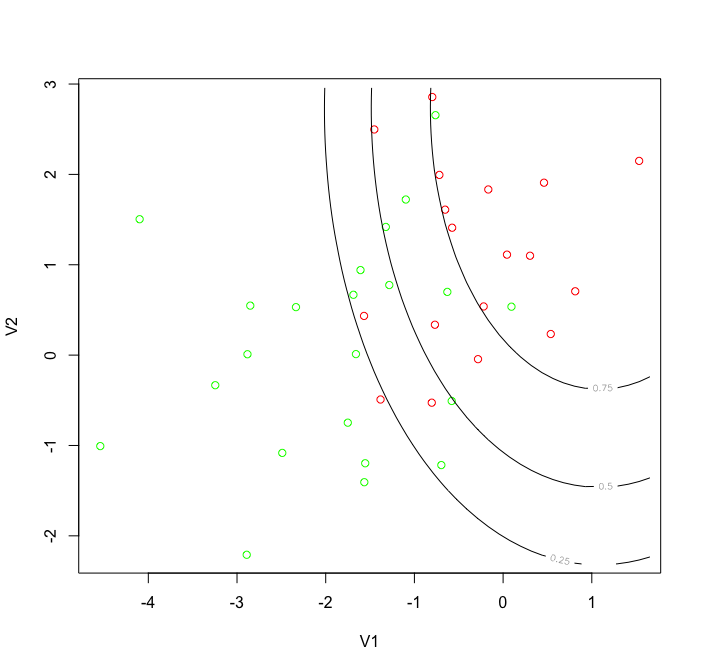
\includegraphics[width=1\linewidth]{img/1-3-verif-adq}
		\caption{\small A. D. Quadratique}
	\end{subfigure}%
	\begin{subfigure}[b]{0.5\linewidth}
		\centering
		\captionsetup{justification=centering, margin=1cm}
		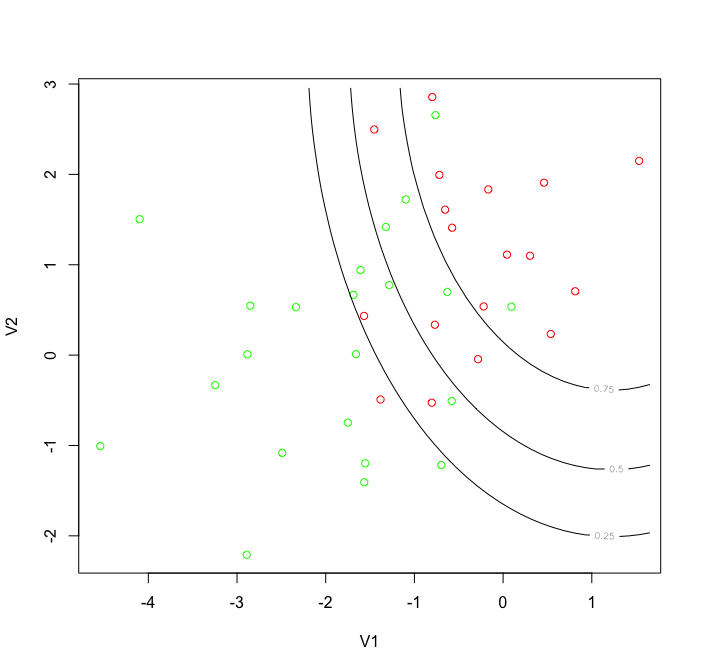
\includegraphics[width=1\linewidth]{img/1-3-verif-nba}
		\caption{\small Classifieur bayésien naïf}
	\end{subfigure}\\%
	\begin{subfigure}[b]{0.5\linewidth}
		\centering
		\captionsetup{justification=centering, margin=1cm}
		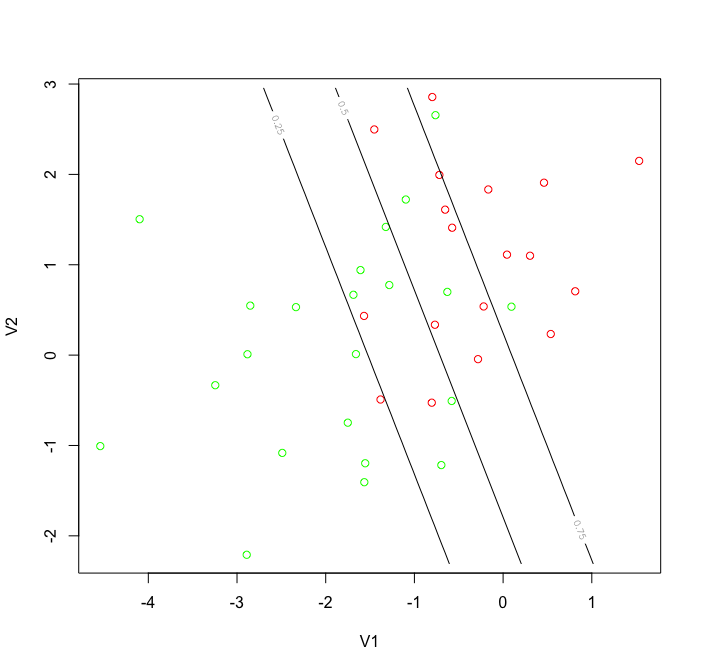
\includegraphics[width=1\linewidth]{img/1-3-verif-adl}
		\caption{\small A. D. Linéaire}
	\end{subfigure}%
	\caption{\small Frontières de décision pour l'analyse discriminante}
	\label{fig:1-3-anadisc}%
\end{figure}


\subsection{Régression logistique}


\begin{figure}[H]
	\centering
	\captionsetup{justification=centering, margin=2cm}
	\begin{subfigure}[b]{0.5\linewidth}
		\centering
		\captionsetup{justification=centering, margin=1cm}
		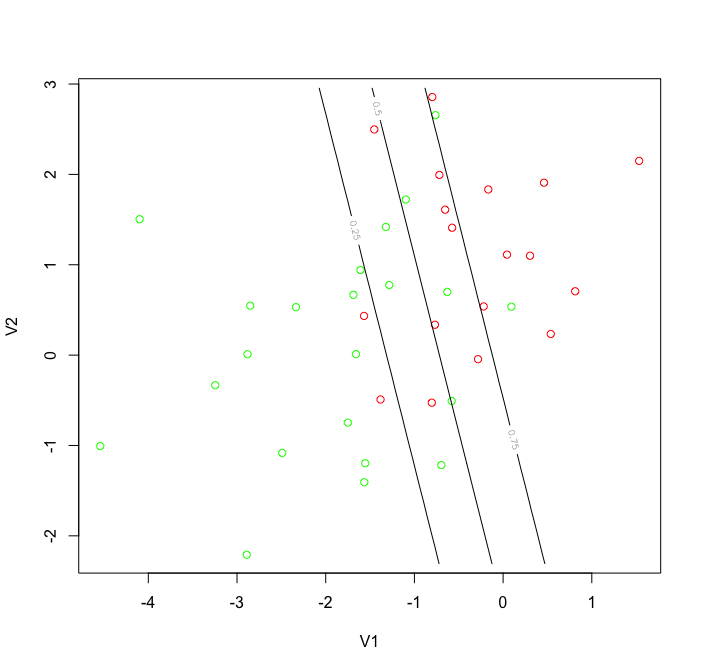
\includegraphics[width=1\linewidth]{img/1-3-verif-log-intercept-true}
		\caption{\small Avec \textit{intercept}}
	\end{subfigure}%
	\begin{subfigure}[b]{0.5\linewidth}
		\centering
		\captionsetup{justification=centering, margin=1cm}
		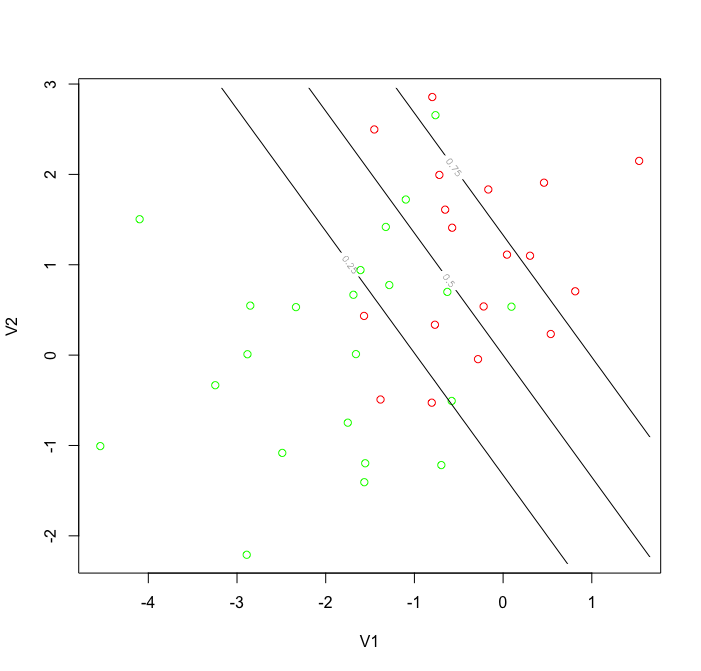
\includegraphics[width=1\linewidth]{img/1-3-verif-log-intercept-false}
		\caption{\small Sans \textit{intercept}}
	\end{subfigure}%
	\caption{\small Frontières de décision pour la régression logistique}
	\label{fig:1-3-log}%
\end{figure}
\begin{figure}[H]
	\centering
	\captionsetup{justification=centering, margin=2cm}
	\begin{subfigure}[b]{0.5\linewidth}
		\centering
		\captionsetup{justification=centering, margin=1cm}
		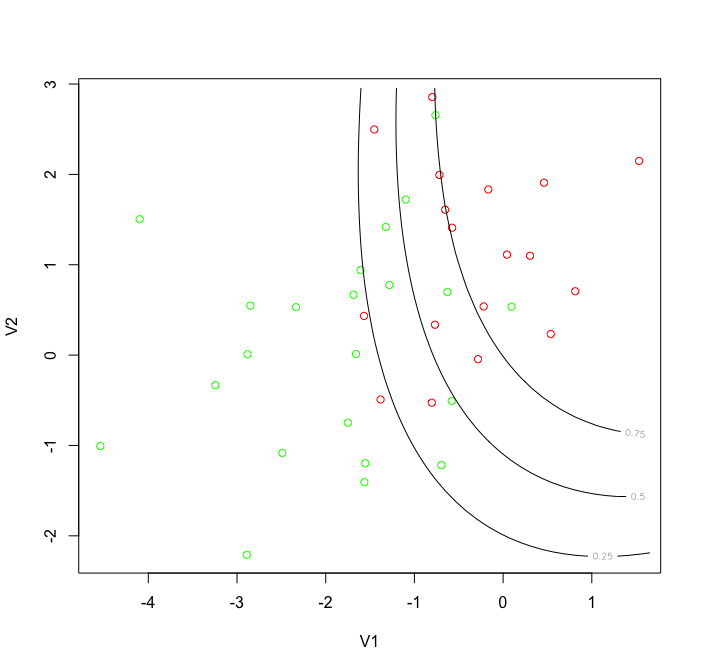
\includegraphics[width=1\linewidth]{img/1-3-verif-log-quad-intercept-true}
		\caption{\small Avec \textit{intercept}}
	\end{subfigure}%
	\begin{subfigure}[b]{0.5\linewidth}
		\centering
		\captionsetup{justification=centering, margin=1cm}
		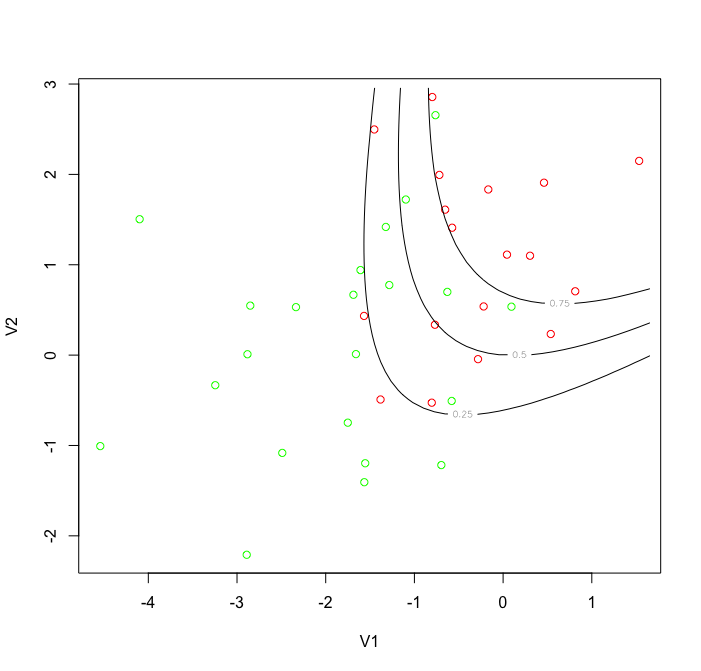
\includegraphics[width=1\linewidth]{img/1-3-verif-log-quad-intercept-false}
		\caption{\small Sans \textit{intercept}}
	\end{subfigure}%
	\caption{\small Frontières de décision pour la régression logistique quadratique}
	\label{fig:1-3-log-quad}%
\end{figure}









\chapter{Application}



On va s'attacher ici à comparer les performances de nos cinq classifieurs~:
\begin{itemize}
	\item Analyse discriminante quadratique, linéaire et bayésien naïf~;
	\item Régression logistique simple et quadratique~;
	\item Arbre de décision.
\end{itemize}

Il est important de bien noter les différence entre ces familles de classifieur, et plus particulièrement entre l'analyse discriminante et les deux autres.\\

L'analyse discriminante \textbf{\textit{suppose}} que les données, conditionnellement à chaque classe $\omega_k$, suivent une loi normale multidimensionnelle d'espérance $\mu_k$ et de variance $\Sigma_k$. En faisant ensuite différentes \textbf{\textit{hypothèses sur ces paramètres}}, on obtient différentes expressions de la règle de Bayes, d'où l'on déduit différentes probabilités à postériori et donc différentes règles de décision en remplaçant les paramètres théoriques par leurs estimations.\\
Dans le cas qui nous intéresse, seules les hypothèses sur les matrices de variances changent en fonction des classifieurs, et donc leurs estimations changent~:
\begin{itemize}
	\item AD Quadratique~: chaque classe $k$ a sa propre matrice de covariance $V_k$~;
	\begin{itemize}
		\item Ce classifieur sera plus fidèle aux les données d'apprentissage et donnera une frontière de décision quadratique~;
		\item Il pourra donc être très efficace dans le cas de classes à distribution quadratique mais risque de faire du sur-apprentissage dans le cas où les données d'apprentissage ne sont pas représentatives des données réelles.
	\end{itemize}
	\item AD Linéaire~: la matrice de covariance est commune à toutes les classes et vaut $\Sigma = \frac{1}{n} \sum_{k=1}^{g} n_k V_k$~;
	\begin{itemize}
		\item Ce classifieur fait une supposition forte qui peut l'amener a avoir de moins bonne performances que l'AD quadratique~;
		\item Par contre, la frontière de décision obtenue étant linéaire, elle sera plus robuste et donc moins sensible au bruit des données (i.e. données d'apprentissage non représentatives).
	\end{itemize}
	\item Classifieur bayésien naïf~: hypothèse d'indépendance conditionnelle des variables, on a alors $\Sigma_k$ égale à la matrice diagonale obtenue à partir des valeurs diagonales de la matrice de covariance $V_k$.
	\begin{itemize}
		\item Ce classifieur propose des frontières de décision quadratique, tout comme l'A.D. quadratique~;
		\item Par contre, l'hypothèse d'indépendance conditionnelle des variables suppose que les classe sont des ellipsoïde dont les axes sont parallèles aux axes du repère.
	\end{itemize}
\end{itemize}

Dans le cas où les données \textit{\textbf{respectent effectivement les hypothèses avancées}} par les classifieurs d'analyse discriminante, alors il est fort probable que ces derniers présentent de bonnes performances. En effet, les estimations des probabilités à postériori seront d'autant plus précises que les hypothèses portant sur la distribution des données sont vérifiées.\\
Mais cela n'est pas obligatoire~: des classes dont les espérances $\mu_k$ sont très proches seront dans la plupart des cas très difficiles à discriminer.\\

La régression logistique \textit{\textbf{ne fait pas d'hypothèses sur les distributions conditionnelles $\mathbf{f_k}$}}~: elle estime directement les probabilités à postériori $\mathbb{P}(\omega_k|x)$ d'appartenance aux classes.\\
La régression logistique simple donnera une frontière de décision linéaire. Lorsqu'on change la dimension des données en rajoutant des variables qui sont des combinaisons des variables originales, la régression logistique devient quadratique et on pourra alors avoir un hyperplan comme frontière de décision.





\section{Test sur les données simulées}


On souhaite comparer les performances de l’analyse discriminante, de la régression logistique (linéaire et quadratique), et des arbres de décision sur les jeux de données simulées \textit{Synth1}, \textit{Synth2} et \textit{Synth3}.\\
Pour ce faire, on répétera $N = 20$ fois pour chaque jeu de données~:
\begin{itemize}
	\item séparer le jeu de données en un ensemble d’apprentissage et un ensemble de test~;
	\item apprendre le modèle sur l’ensemble d’apprentissage~;
	\item effectuer le classement des données de test et calculer le taux d’erreur associé.
\end{itemize}

Pour chaque jeu de données, on calculera ensuite le taux d’erreur (de test) moyen $\hat{\epsilon}$ sur les $N = 20$ séparations effectuées.


\subsection{Visualisation graphique des données}

Les données synthétiques sont de dimension $p = 2$, ce qui nous permet d'en tracer une visualisation graphique simple. Cette visualisation nous donnera des intuitions quand aux modèles de discrimination qui pourront être efficaces ou non sur ces données.


\begin{figure}[H]
	\centering
	\captionsetup{justification=centering, margin=2cm}
	\begin{subfigure}[b]{0.5\linewidth}
		\centering
		\captionsetup{justification=centering, margin=1cm}
		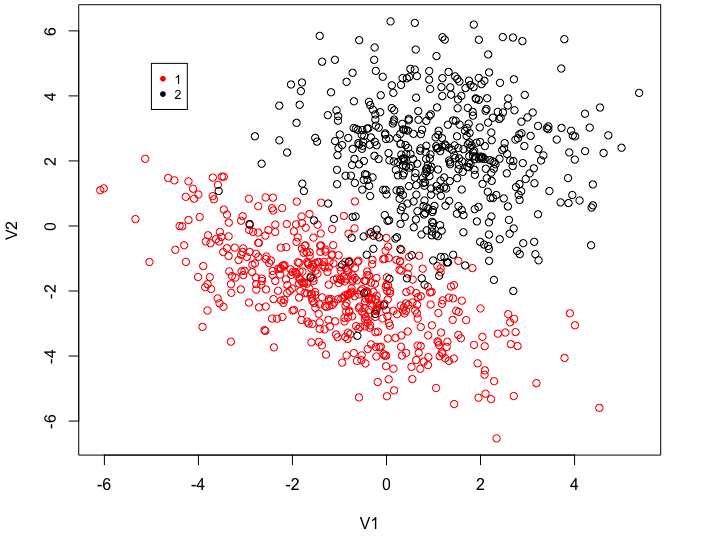
\includegraphics[width=1\linewidth]{img/2-1-1-synth1-visualisation}
		\caption{\small Données synthétiques \textit{Synth1}}
	\end{subfigure}%
	\begin{subfigure}[b]{0.5\linewidth}
		\centering
		\captionsetup{justification=centering, margin=1cm}
		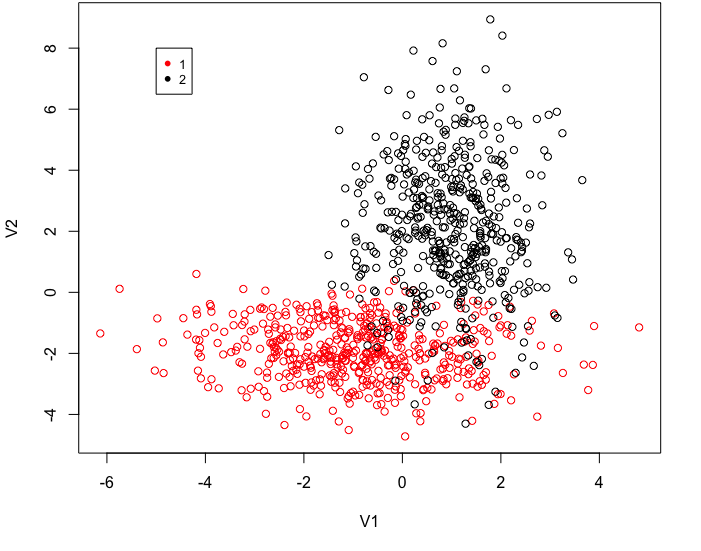
\includegraphics[width=1\linewidth]{img/2-1-1-synth2-visualisation}
		\caption{\small Données synthétiques \textit{Synth2}}
	\end{subfigure}\\%
	\begin{subfigure}[b]{0.5\linewidth}
		\centering
		\captionsetup{justification=centering, margin=1cm}
		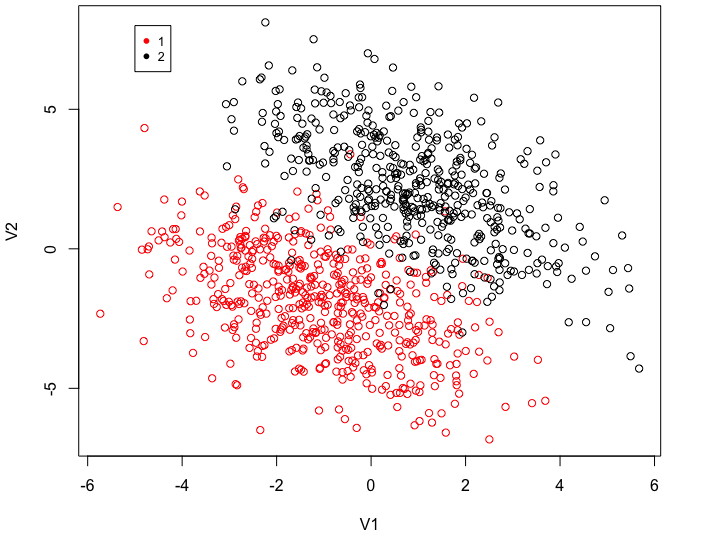
\includegraphics[width=1\linewidth]{img/2-1-1-synth3-visualisation}
		\caption{\small Données synthétiques \textit{Synth3}}
	\end{subfigure}%
	\caption{\small Visualisation des données synthétiques \textit{Synth1}, \textit{Synth2} et \textit{Synth3}}
	\label{fig:2-1-1-synth-visualisation}%
\end{figure}

~\\
Remarques possibles suite à la visualisation~:
\begin{itemize}
	\item Données \textit{Synht1}~:
	\begin{itemize}
		\item Classes dont les variances $\Sigma$ semblent différentes, $\Sigma_1$ donnant une forme d'ellipsoïde non parallèle aux axes quand $\Sigma_2$ semble définir une classe plutôt circulaire~;
		\item Il semble y avoir peu de chevauchement entre les classes~;
		\item Compte tenu de leurs formes, un classifieur à frontière de décision quadratique tendra à être plus efficace qu'un classifieur à frontière de décision linéaire.
	\end{itemize}
	\item Données \textit{Synht2}~:
	\begin{itemize}
		\item Classes dont les variances $\Sigma$ semblent inversées~: la classe $\omega_1$ est très étendues sur l'axe V1 quand la classe $\omega_1$ est très étendue sur l'axe V2~;
		\item Le chevauchement entre les classes est plus important que dans les deux autres jeux de données~;
		\item De façon plus prononcée que pour \textit{Synth1} ou \textit{Synth3}, un classifieur à frontière de décision quadratique sera plus performant qu'un classifieur à frontière de décision linéaire.
	\end{itemize}
	\item Données \textit{Synht3}~:
	\begin{itemize}
		\item Classes dont les variances $\Sigma$ semblent identiques~;
		\item Peu de chevauchement entre les classes~;
		\item L'analyse discriminante linéaire semble particulièrement indiquée ici. On peut même s'attendre à ce que les frontières de décision quadratiques aient une forme quasiment linéaire.
	\end{itemize}
	\item Classifieur des arbres de décision~:
		\begin{itemize}
			\item Les classes se présentant visuellement sous forme d'ellipsoïdes (pas toujours parallèles aux axes), ce classifieur~–~proposant un frontière de décision linéaire par morceaux \textbf{et} parallèle aux axes des dimensions (= variables)~–~pourra logiquement donner de plus mauvais résultats que les autres sur ces jeux de données.
		\end{itemize}
\end{itemize}


\subsection{Visualisation "mathématique" des données via l'estimation des paramètres}
\label{subsection:analyse-parametres-donnees-synthetiques}


\begin{table}[H]
	\centering
	\begin{tabular}{c|c|c|c}
		Fichier source & Centres de gravité $\mu$ & Variances $\Sigma$ & Proportions $\pi$ \\ 
		\hline
		\small Synth1 
		& 	$\mu_{1} = 
		\begin{pmatrix}
		-1.03 \\ 
		-1.95
		\end{pmatrix} $ , 
		$\mu_{2} = 
		\begin{pmatrix}
		1.10 \\ 
		2.07
		\end{pmatrix} $ 
		&  	$\Sigma_{1} = 
		\begin{pmatrix}
		2.89 & -1.53 \\
		-1.53 & 1.96\\
		\end{pmatrix} $ , 
		$\Sigma_{2} = 
		\begin{pmatrix}
		2.09 & 0.00\\
		0.00 & 2.81 \\
		\end{pmatrix} $
		& 	$\begin{pmatrix} 
		\pi_{1} = 0.51\\
		\pi_{2} = 0.49
		\end{pmatrix}$\\ 
		\hline
		\small Synth2
		& 	$\mu_{1} = 
		\begin{pmatrix}
		-0.90   \\ 
		-1.92
		\end{pmatrix} $ , 
		$\mu_{2} = 
		\begin{pmatrix}
		0.97  \\ 
		2.17
		\end{pmatrix} $ 
		&  	$\Sigma_{1} = 
		\begin{pmatrix}
		2.81 & -0.19\\
		-0.19 &  0.90\\
		\end{pmatrix} $ , 
		$\Sigma_{2} = 
		\begin{pmatrix}
		0.90 & -0.04\\
		-0.04 & 4.60\\
		\end{pmatrix} $
		& 	$\begin{pmatrix} 
		\pi_{1} = 0.5\\
		\pi_{2} = 0.5
		\end{pmatrix}$\\ 
		\hline
		\small Synth3
		& 	$\mu_{1} = 
		\begin{pmatrix}
		-1.06  \\ 
		-1.91 
		\end{pmatrix} $ , 
		$\mu_{2} = 
		\begin{pmatrix}
		0.92  \\ 
		2.19 
		\end{pmatrix} $ 
		&  	$\Sigma_{1} = 
		\begin{pmatrix}
		2.88 & -1.55\\
		-1.55 & 3.50\\
		\end{pmatrix} $ , 
		$\Sigma_{2} = 
		\begin{pmatrix}
		2.92 & -2.02\\
		2.02 & 4.17\\
		\end{pmatrix} $
		& 	$\begin{pmatrix} 
		\pi_{1} = 0.52\\
		\pi_{2} = 0.48
		\end{pmatrix}$\\
	\end{tabular}
	\caption{\small Paramètres estimés des fichiers \textit{Synth1}, \textit{Synth2} et \textit{Synth3}}
	\label{table:1-2-parametres-Synth1}
\end{table}

Remarques~:
\begin{itemize}
	\item Données \textit{Synht1}~:
	\begin{itemize}
		\item Comme nous en avons eu l'intuition précédemment lors de la visualisation, on a bien $\Sigma_{1} \neq \Sigma_{2}$ avec $\omega_1$ légèrement plus dispersée sur l'axe V1 après rotation et $\omega_2$ légèrement plus dispersée sur l'axe V2 (et non circulaire comme on l'avait supposé)~;
		\item Compte tenu des paramètres estimés, la classification discriminante quadratique sera plus indiquée que la linéaire ou le classifieur bayésien naïf, car leurs hypothèses ne sont pas vérifiées~;
		\begin{itemize}
			\item Par équivalence, la régression logistique quadratique sera plus indiquée que la régression logistique simple.
		\end{itemize}
	\end{itemize}
	\item Données \textit{Synht2}~:
	\begin{itemize}
		\item Compte tenu des paramètres estimés, le classifieur bayésien naïf sera plus indiqué que la discrimination linéaire ou quadratique, car il semble bien qu'on ait l'hypothèse d'indépendance conditionnelle des variables vérifiée (covariances nulles ou insignifiantes dans les matrices $\Sigma_k$)~;
		\begin{itemize}
			\item Par équivalence, la régression logistique quadratique sera plus indiquée que la régression logistique simple (le classifieur bayésien naïf donne une frontière de décision quadratique).
		\end{itemize}
	\end{itemize}
	\item Données \textit{Synht3}~:
	\begin{itemize}
		\item Compte tenu des paramètres estimés, l'analyse discriminante linéaire semble la plus indiquée. Même si les matrices $\Sigma_{1}$ et $\Sigma_{2}$ ne sont pas exactement égales entre-elles, elles sont tout de même relativement proches~;
		\begin{itemize}
			\item Par équivalence, la régression logistique simple sera plus indiquée que la régression logistique quadratique.
		\end{itemize}
	\end{itemize}

\end{itemize}

\subsection{Frontières de décisions}

Des exemples de frontières de décisions sont disponibles en annexe~:
\begin{itemize}
	\item Données \textit{Synht1}~: voir \autoref{appendix:front-decision-synth-1}~;
	\item Données \textit{Synht2}~: voir \autoref{appendix:front-decision-synth-2}~;
	\item Données \textit{Synht3}~: voir \autoref{appendix:front-decision-synth-3}.
\end{itemize}



\subsection{Calculs des taux d'erreur}

\textit{\textbf{Remarque sur l'espérance et la variance du taux d'erreur $\hat{\epsilon}$}~: on va par la suite calculer ces statistiques à des fins analytiques. Il faut prendre note que nous allons les calculer sur un échantillon de taille $n=6$, voire moins lorsqu'on comparera les différents types de classifieur. Bien que donnant certaines indications et servant notre propos lors des comparaisons, ces statistiques doivent être considérées avec prudence.}\\

Calcul du taux d'erreur $\hat{\epsilon}$ sur les données synthétiques~:
\begin{table}[H]
	\centering
	\captionsetup{justification=centering, margin=4cm}
	\begin{tabular}{c|c|c|c|c|c|c}
		Fichier source & ADQ & ADL & NBA & Log & Log Quad & Tree \\ 
		\hline
		Synth1 & \textbf{3.43} & 4.52 & 4.22 & 3.67 & \textbf{3.25} & 4.73  \\ 
		Synth2 & 6.23 & 8 & \textbf{6.17} & 6.85 & \textbf{6.44} & 8.09  \\ 
		Synth3 & 4.23 & \textbf{4.16} & 5.45 & \textbf{4.2} & 4.37 & 5.93  \\ 
	\end{tabular}
	\caption{\small Estimation du taux d'erreur $\hat{\epsilon}$ sur $N=20$ itérations des différents classifieurs sur les données synthétiques}
	\label{table:2-1-erreur-data-synth}
\end{table}

Comme on avait pu le supposer précédemment lors de l'analyse des visualisations graphiques et des paramètres des classes, on a bien pour~:
\begin{itemize}
	\item Données \textit{Synht1}~:
	\begin{itemize}
		\item De meilleures performances avec l'analyse discriminante quadratique et la régression logistique quadratique.
	\end{itemize}
	\item Données \textit{Synht2}~:
	\begin{itemize}
		\item De meilleures performances avec le classifieur bayésien naïf et la régression logistique quadratique.
	\end{itemize}
	\item Données \textit{Synht3}~:
	\begin{itemize}
		\item De meilleures performances avec l'analyse discriminante linéaire et la régression logistique simple.
	\end{itemize}
	\item Classifieur des arbres de décision~:
	\begin{itemize}
		\item Les plus mauvaises performance pour chaque jeu de données.
	\end{itemize}
\end{itemize}




Il faut néanmoins nuancer nos propos car les performances des classifieurs par fichier sont à première vue sensiblement les mêmes (faible variance)~:
\begin{table}[H]
	\centering
	\captionsetup{justification=centering, margin=4cm}
	\begin{tabular}{c|c|c}
		Fichier source & Espérance de $\hat{\epsilon}$ & Variance de $\hat{\epsilon}$  \\ 
		\hline
		Synth1 & 3.97 & 0.37 \\ 
		Synth2 & 6.96 & 0.76  \\ 
		Synth3 & 4.72 & 0.59  \\ 
	\end{tabular}
	\caption{\small Espérances et variances des taux d'erreurs de tous les classifieurs pour un fichier synthétique donné}
	\label{table:2-1-erreur-data-synth-mean-var}
\end{table}



\textit{\textbf{Remarque}~: dans la suite de l'analyse des performances des classifieurs, on laissera de côté l'arbre de décision. Ce dernier propose une frontière linéaire parallèle aux axes "par morceaux" (voir frontières de décision en annexe \autoref{fig:front-decision-synth-1-tree}, \autoref{fig:front-decision-synth-2-tree} et \autoref{fig:front-decision-synth-3-tree}) et donne les résultats les plus mauvais, comparativement aux autres classifieurs.\\
Les données étant distribuées de façon ellipsoïdale, il n'est pas étonnant que ce soit ce classifieur qui présente la plus mauvaise performance.}\\

Nous nous proposons maintenant de faire une analyse comparative des performances en deux parties~:
\begin{itemize}
	\item les modèles d'analyse discriminante comparés à la régression logistique~;
	\item les modèles à frontière de décision linéaire comparés aux modèles à frontière de décision quadratique.
\end{itemize}

\subsubsection{Comparaison du taux d'erreur $\hat{\epsilon}$ entre analyse discriminante et régression logistique}

\begin{table}[H]
	\centering
	\captionsetup{justification=centering, margin=3cm}
	\begin{tabular}{c|c|c|c|c}
		Fichier source & AD~: $\mathbb{E}\ [\ \hat{\epsilon}\ ]$ & AD~: $Var\ [\ \hat{\epsilon}\ ]$ & RL~: $\mathbb{E}\ [\ \hat{\epsilon}\ ]$ & RL.~: $Var\ [\ \hat{\epsilon}\ ]$ \\ 
		\hline
		Synth1 & 4.06  & 0.32  & \textbf{3.46}  & \textbf{0.09}  \\ 
		Synth2 & 6.8  & 1.08 & \textbf{6.64}  & \textbf{0.08} \\ 
		Synth3 & 4.61 & 0.53 & \textbf{4.29}  & \textbf{0.01}  \\ 
	\end{tabular}
	\caption{\small Espérances et variances des taux d'erreurs des classifieurs de type analyse discriminante versus les classifieurs de type régression logistique}
	\label{table:2-1-erreur-data-synth-mean-var-ad-vs-regression}
\end{table}

Étonnamment, et quand bien même les données suivent dans chaque classe une loi normale multivariée et respectent à tour de rôle les hypothèses d'un classifieur d'analyse discriminante donné, on a quand même des performances \textit{légèrement} supérieures pour la régression logistique (simple ou quadratique). Mais cette différence est tout de même trop faible pour être significative (0.35 d'écart en moyenne).\\
La variance du taux d'erreur est par contre significativement plus faible pour la régression logistique. Cela peut s'expliquer par le fait que cette dernière \textit{\textbf{ne fait pas de supposition}} sur la distribution des données, contrairement à l'analyse discriminante.

\subsubsection{Comparaison du taux d'erreur $\hat{\epsilon}$ entre classifieurs à frontière de décision linéaire ou quadratique}
\begin{table}[H]
	\centering
	\captionsetup{justification=centering, margin=1cm}
	\begin{tabular}{c|c|c|c|c}
		Fichier source & Front. Lin~: $\mathbb{E}\ [\ \hat{\epsilon}\ ]$ & Front. Lin~: $Var\ [\ \hat{\epsilon}\ ]$ & Front. Quad~: $\mathbb{E}\ [\ \hat{\epsilon}\ ]$ & Front. Quad.~: $Var\ [\ \hat{\epsilon}\ ]$ \\ 
		\hline
		Synth1 & 4.09    & 0.36   & \textbf{3.63}   & \textbf{0.27}   \\ 
		Synth2 & 7.42   & 0.66   &  \textbf{6.28}  & \textbf{0.02}  \\ 
		Synth3 &  \textbf{4.18}  &  \textbf{0}  & 4.68   & 0.45   \\ 
	\end{tabular}
	\caption{\small Espérances et variances des taux d'erreurs des classifieurs donnant une frontière de décision linéaire versus les classifieurs donnant une frontière de décision quadratique}
	\label{table:2-1-erreur-data-synth-mean-var-lin-vs-quad}
\end{table}

Cette comparaison renforce les hypothèses émises précédemment lors de l'analyse des paramètres estimés des classes (voir \autoref{subsection:analyse-parametres-donnees-synthetiques})~:
\begin{itemize}
	\item Les modèles quadratiques proposant des frontières de décision quadratiques sont plus performants sur les données \textit{Synth1} et \textit{Synth2}~;
	\item Les modèles linéaires proposant des frontières de décision linéaires sont plus performants sur les données \textit{Synth3}.
\end{itemize}

On remarquera aussi en observant les variances que les modèles les plus adéquats sont aussi les plus fiables, c'est à dire les plus stables dans leurs performances~: leurs variances sont systématiquement plus faibles que celles des modèles non adéquats.

\section{Test sur données réelles}


\subsection{Données "Pima"}

\begin{table}[H]
	\centering
	\captionsetup{justification=centering, margin=4cm}
	\begin{tabular}{c|c|c|c|c|c|c}
		Fichier source & ADQ & ADL & NBA & Log & Log Quad & Tree \\ 
		\hline
		Pima & 23.97 & 22.62 & 23.8 & 21.77 & 24.72 & 26.23  \\ 
	\end{tabular}
	\caption{\small Estimation du taux d'erreur sur $N=100$ itérations des différents classifieurs sur les données "Pima"}
	\label{table:2-1-erreur-data-pima}
\end{table}

\subsection{Données "Breast Cancer Wisconsin"}

\begin{table}[H]
	\centering
	\captionsetup{justification=centering, margin=4cm}
	\begin{tabular}{c|c|c|c|c|c}
		Fichier source & ADQ & ADL & NBA & Log & Tree \\ 
		\hline
		Brestcancer & 4.93 & 4.46 & 3.99 & 3.94 & 5.39 \\ 
	\end{tabular}
	\caption{\small Estimation du taux d'erreur sur $N=100$ itérations des différents classifieurs sur les données "breast cancer Wisconsin"}
	\label{table:2-1-erreur-data-breastcancer}
\end{table}
























\chapter{Challenge : données "Spam"}








































\appendix


\chapter{Fonctions pour l'analyse discriminante}
\label{appendix:functions-ana-disc}

\section{Fonctions d'apprentissage \texttt{adq.app}, \texttt{adl.app} et \texttt{nba.app}}
\label{appendix:functions-ana-disc-app}

\subsubsection{Fonctions utilitaires de calcul des proportions, moyennes et matrices de co-variance}

\begin{figure}[H]
	\centering
	\captionsetup{justification=centering, margin=3cm}
	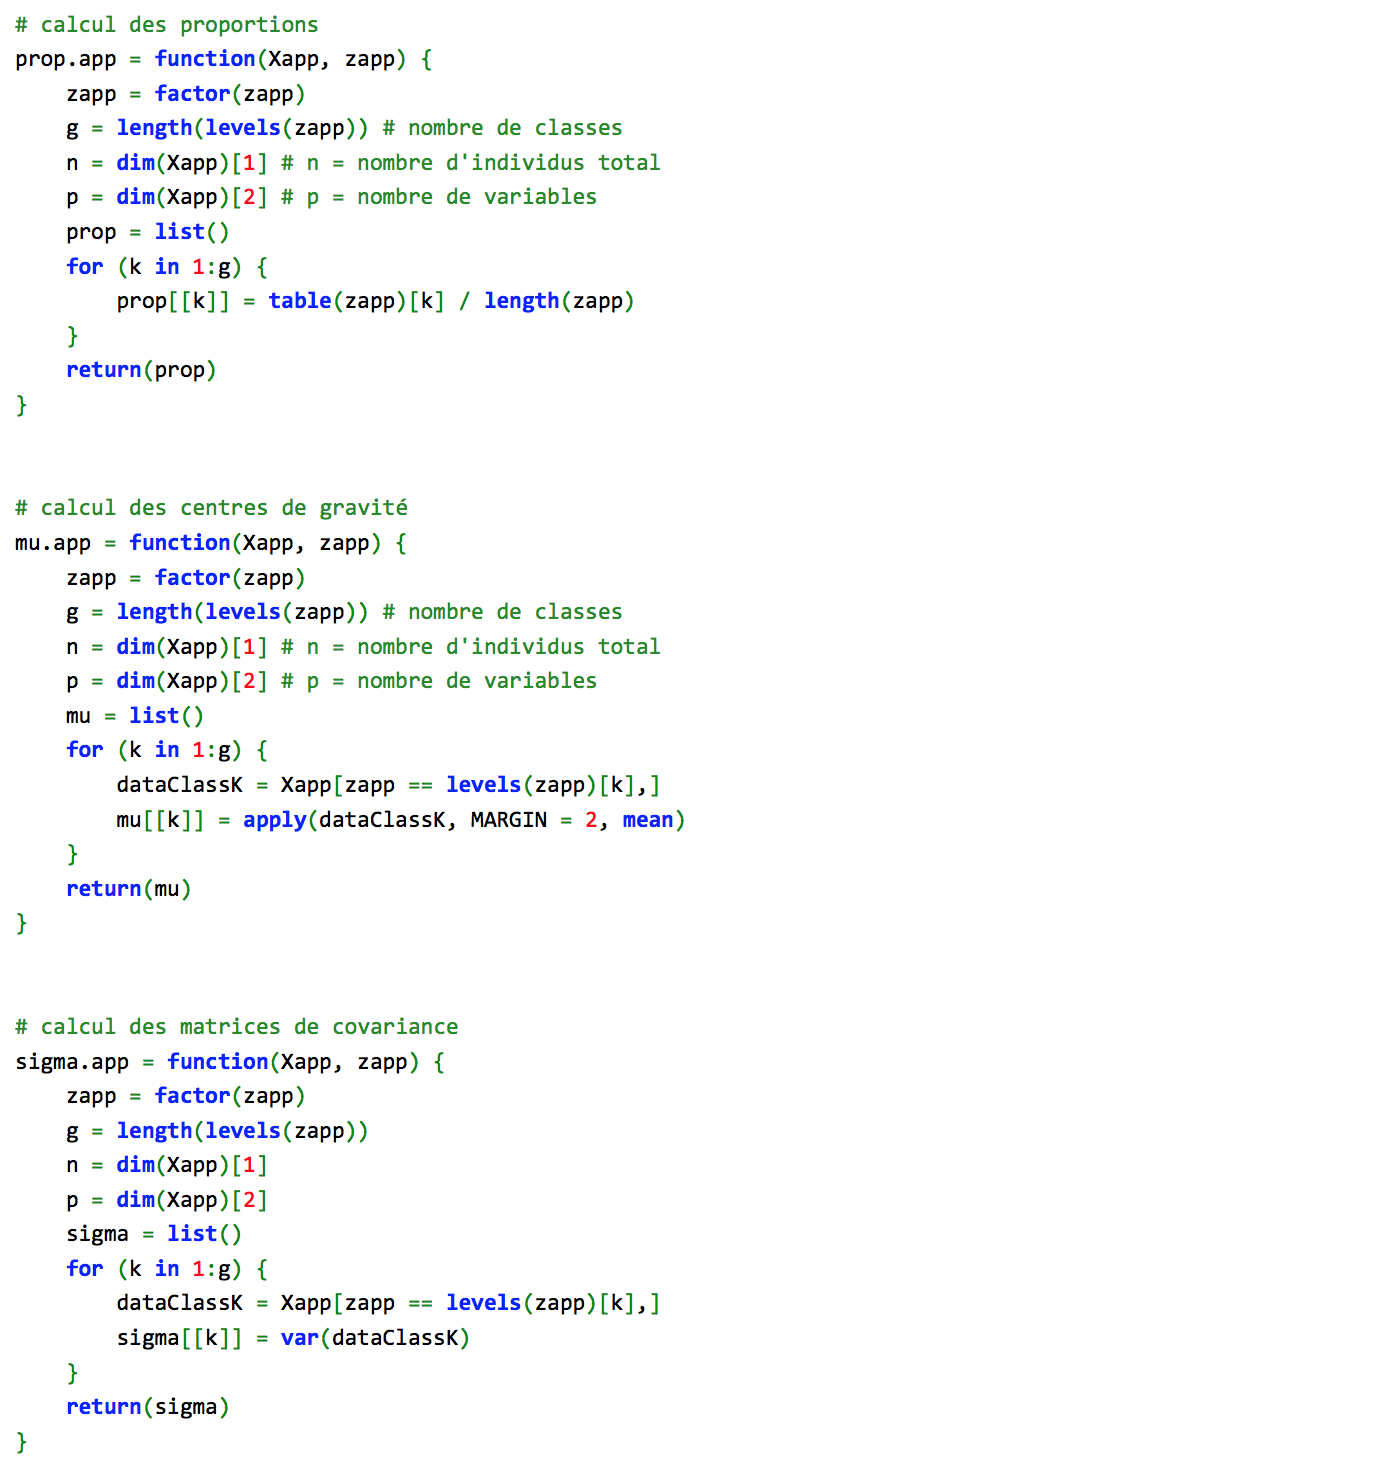
\includegraphics[width=0.9\linewidth]{img/A-anadisc-sub-functions}
%	\caption{}
	\label{fig:A-1-anadisc-sub-functions}
\end{figure}

\subsubsection{Fonctions d'apprentissage des paramètres}

\begin{figure}[H]
	\centering
	\captionsetup{justification=centering, margin=3cm}
	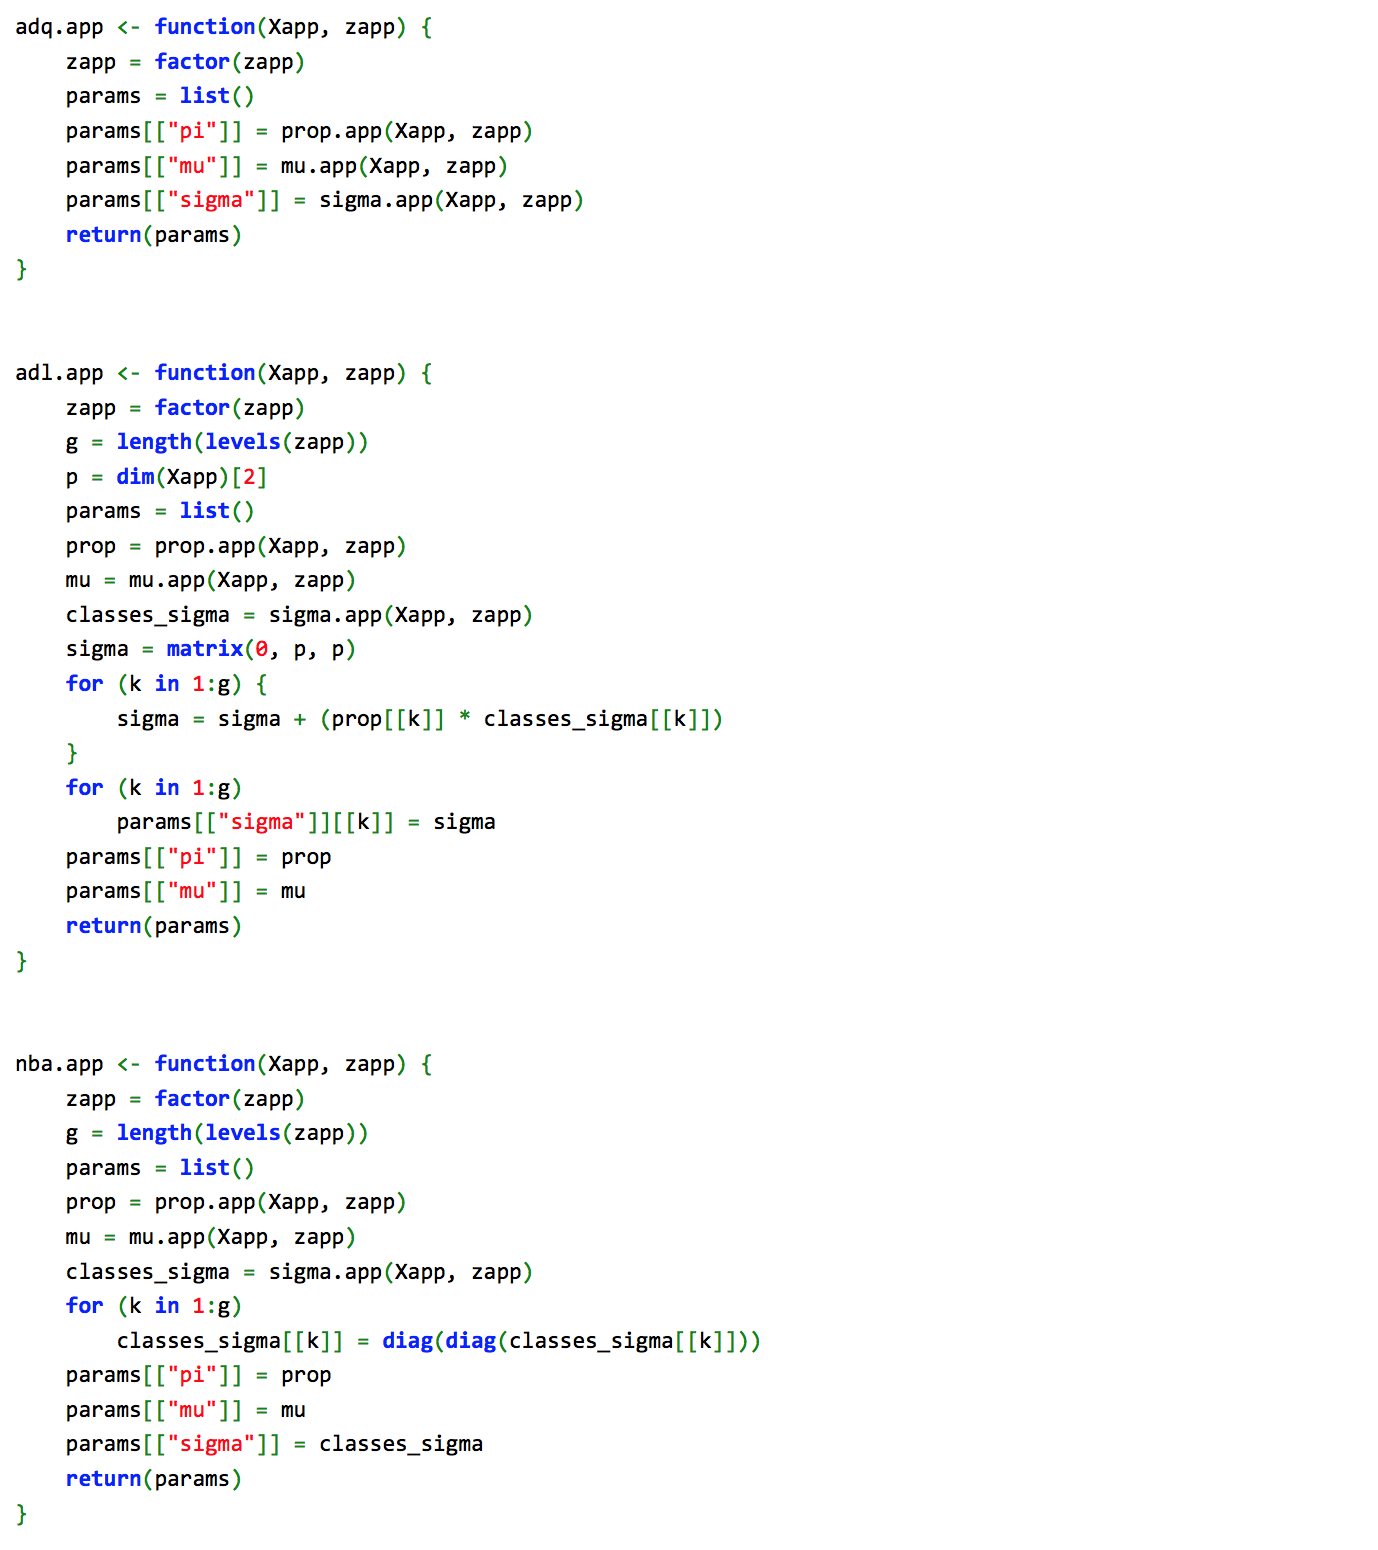
\includegraphics[width=0.9\linewidth]{img/A-anadisc-app-functions}
	%	\caption{}
	\label{fig:A-1-anadisc-app-functions}
\end{figure}

\section{Fonction de discrimination \texttt{ad.val}}
\label{appendix:functions-ana-disc-val}
\begin{figure}[H]
	\centering
	\captionsetup{justification=centering, margin=3cm}
	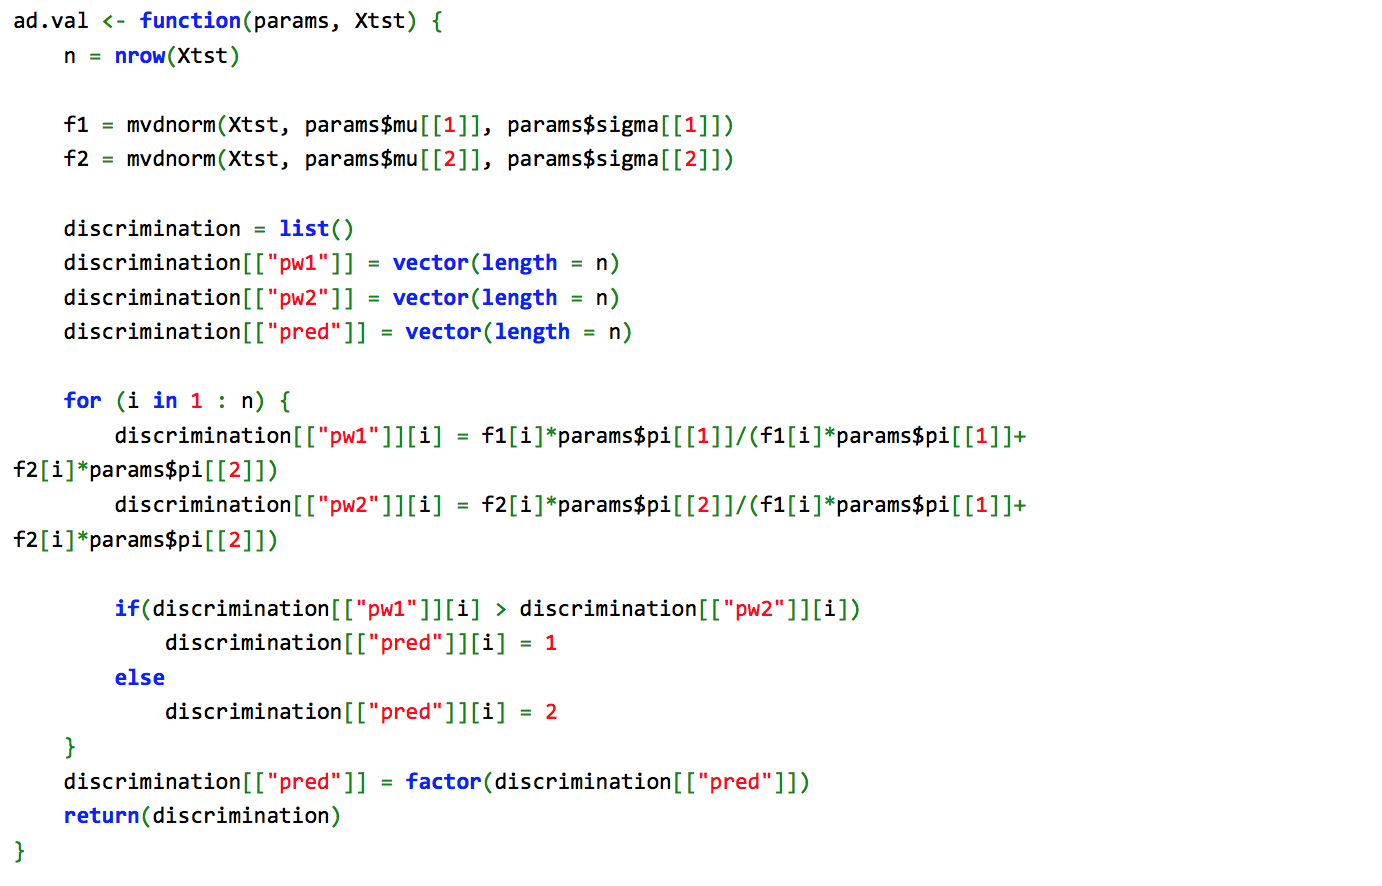
\includegraphics[width=0.9\linewidth]{img/A-anadisc-val-functions}
	%	\caption{}
	\label{fig:A-1-anadisc-val-functions}
\end{figure}



\chapter{Fonctions pour la régression logistique}
\label{appendix:functions-reg-log}

\section{Fonction de calcul des probabilités à postériori \texttt{postprob}}
\label{appendix:functions-reg-log-postprob}

\begin{figure}[H]
	\centering
	\captionsetup{justification=centering, margin=3cm}
	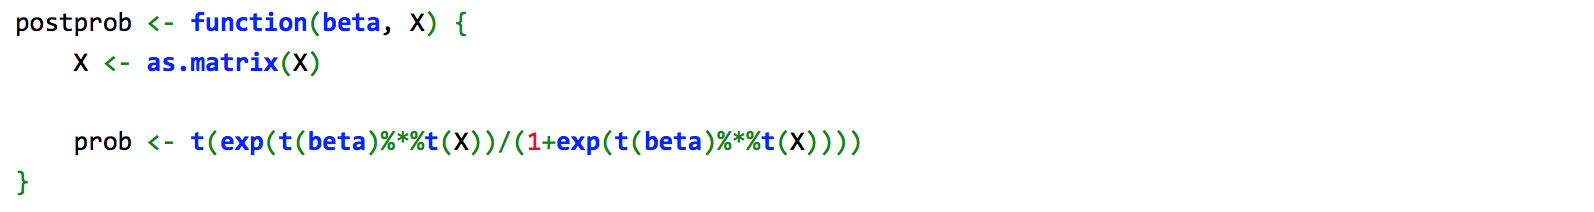
\includegraphics[width=0.9\linewidth]{img/B-log-post-prob-function}
	%	\caption{}
	\label{fig:B-log-post-prob-function}
\end{figure}

\section{Fonction d'apprentissage \texttt{log.app}}
\label{appendix:functions-reg-log-simple-app}

\begin{figure}[H]
	\centering
	\captionsetup{justification=centering, margin=3cm}
	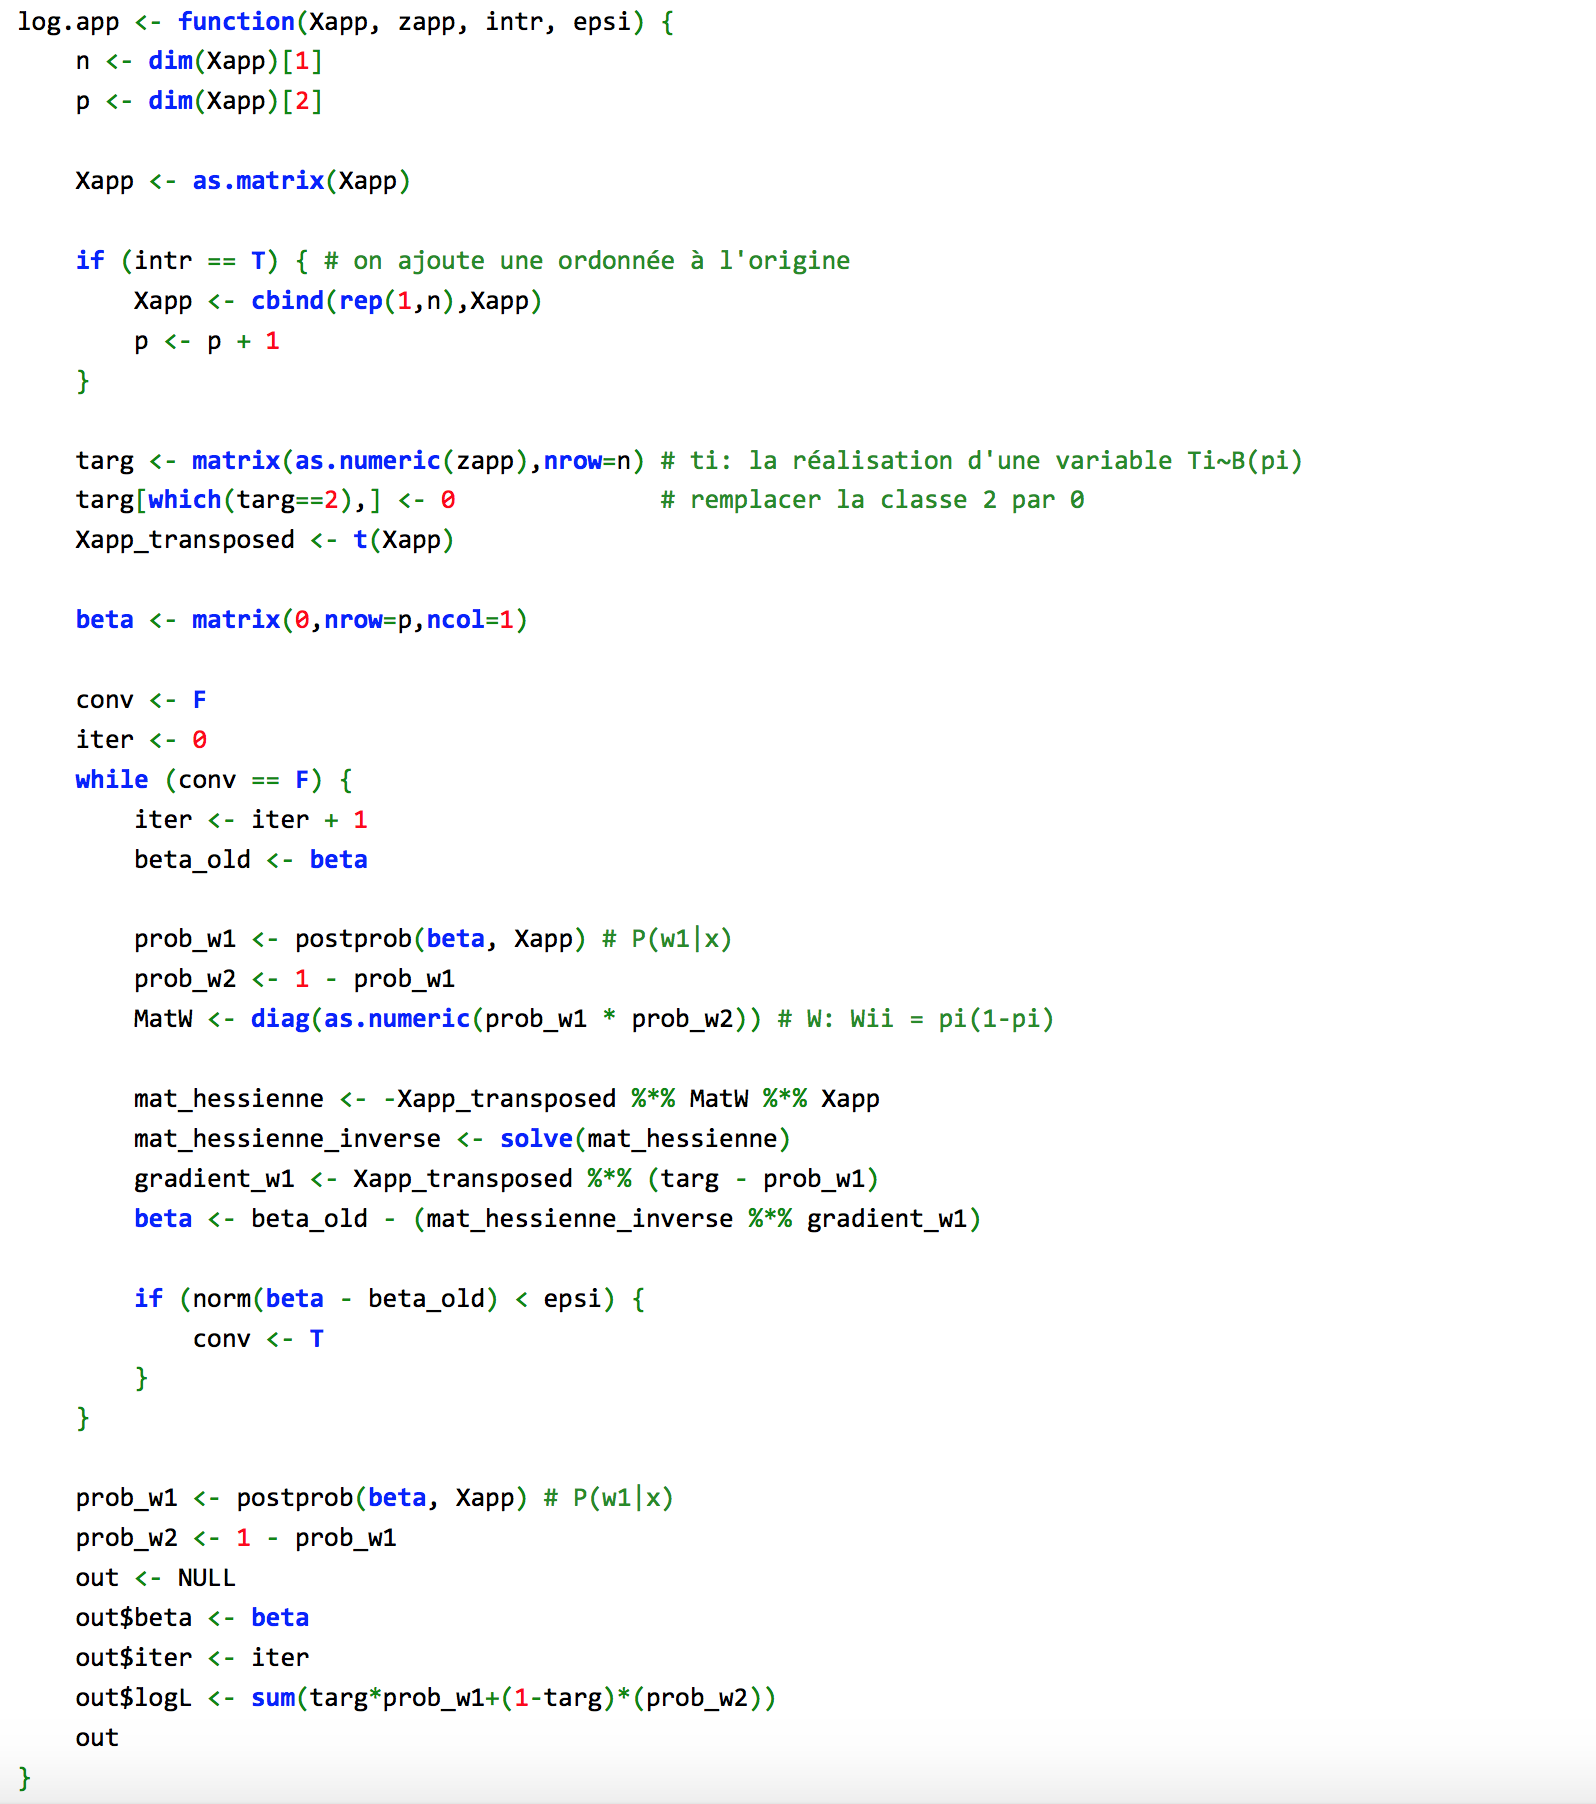
\includegraphics[width=0.9\linewidth]{img/B-log-app-function}
	%	\caption{}
	\label{fig:B-log-app-function}
\end{figure}

\section{Fonction de discrimination \texttt{log.val}}
\label{appendix:functions-reg-log-simple-val}

\begin{figure}[H]
	\centering
	\captionsetup{justification=centering, margin=3cm}
	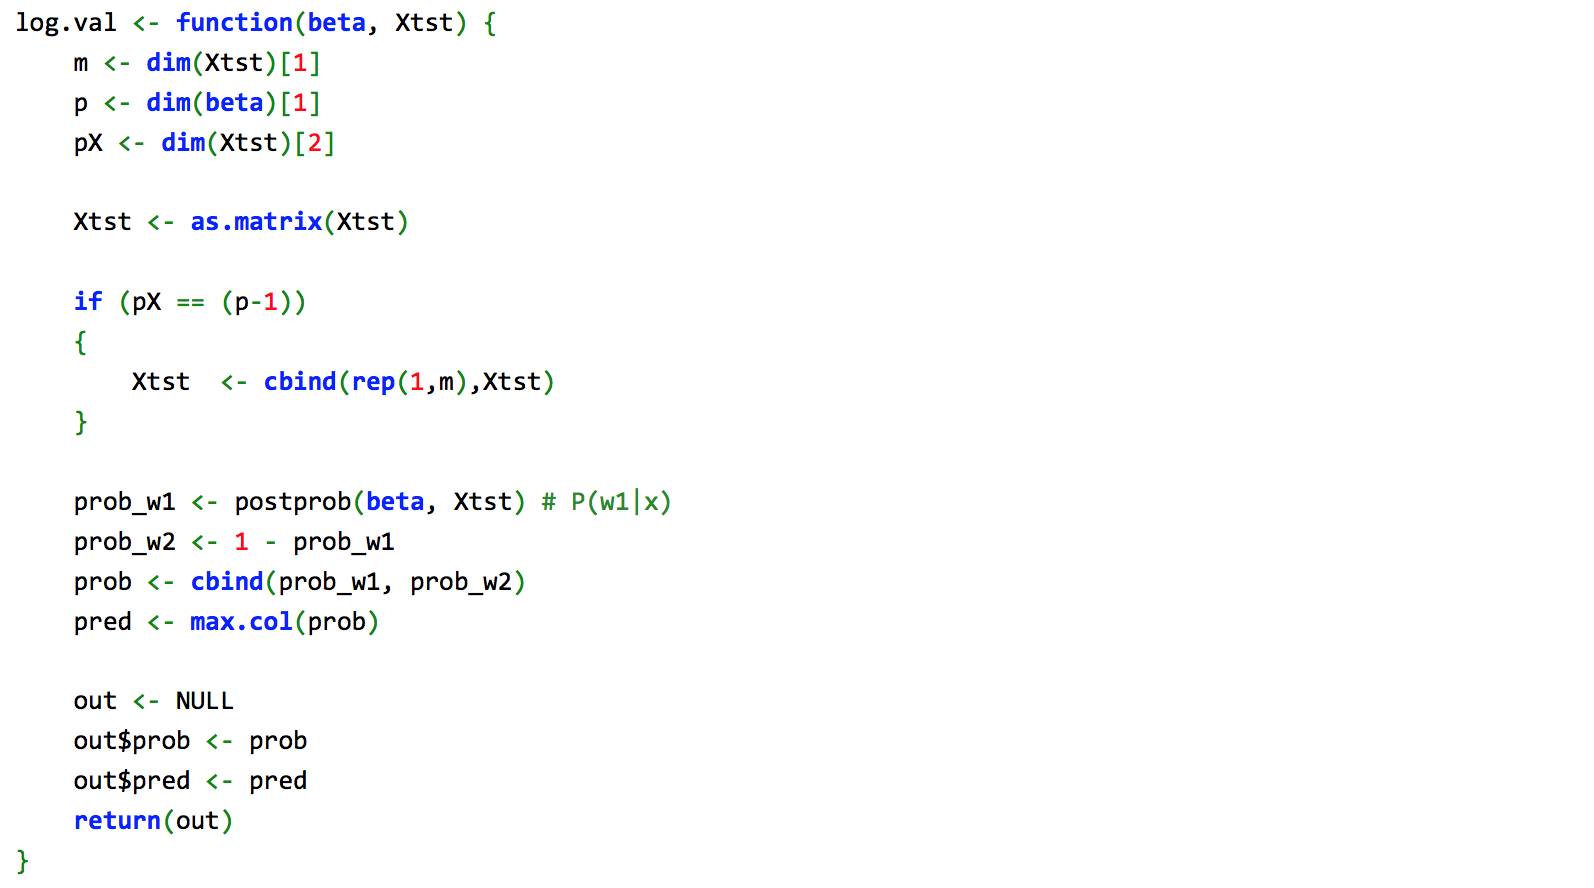
\includegraphics[width=0.9\linewidth]{img/B-log-val-function}
	%	\caption{}
	\label{fig:B-log-val-function}
\end{figure}

\section{Fonction pour la régression logistique quadratique}
\label{appendix:functions-reg-log-quad}

Fonction qui transforme l'espace de X en un espace quadratique~:
\begin{figure}[H]
	\centering
	\captionsetup{justification=centering, margin=3cm}
	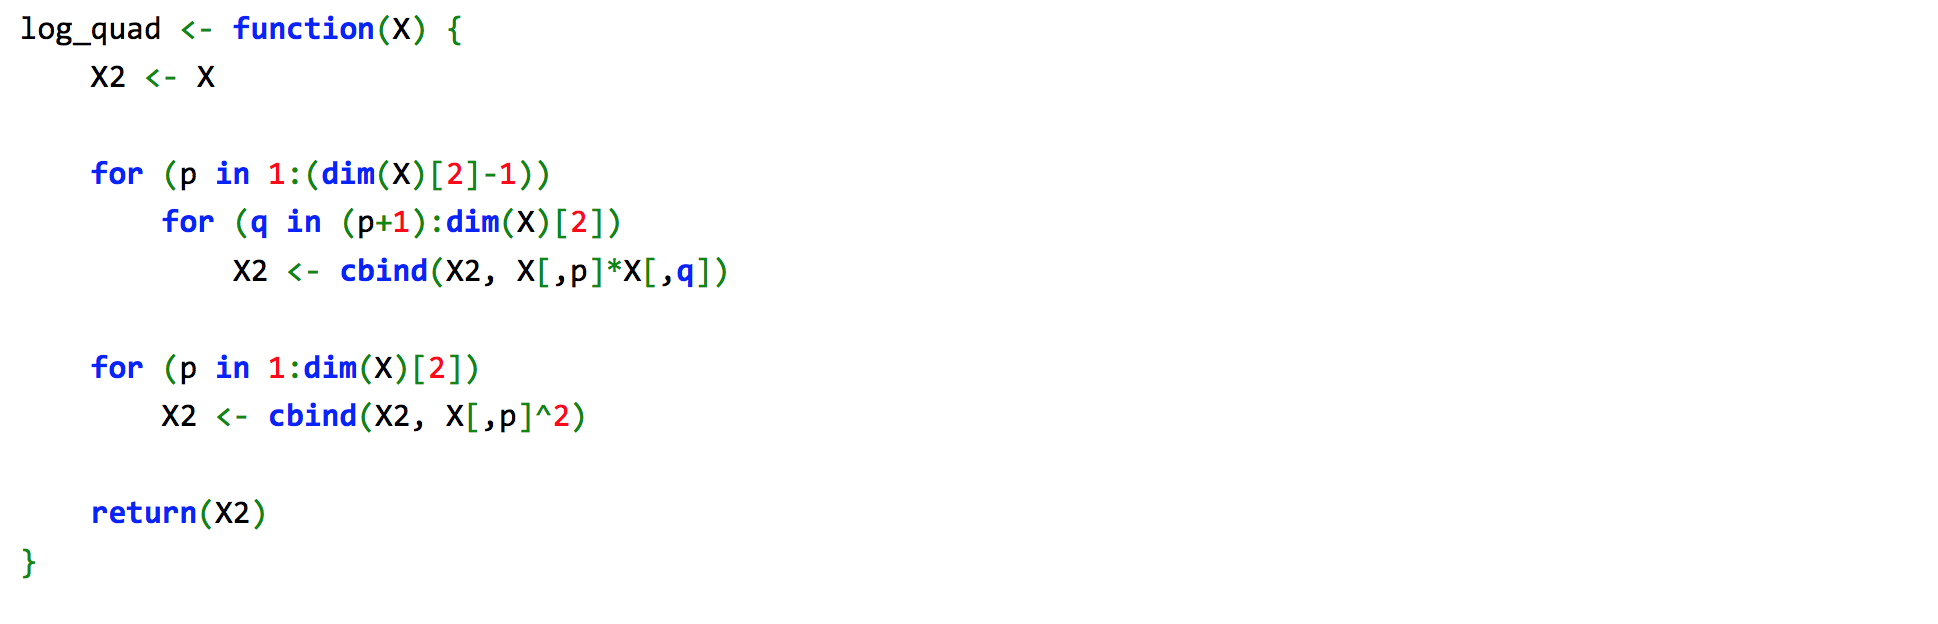
\includegraphics[width=0.9\linewidth]{img/B-log-quad-function}
	%	\caption{}
	\label{fig:B-log-quad-function}
\end{figure}



\chapter{Frontières de décision}

\section{Données \textit{Synth1}}
\label{appendix:front-decision-synth-1}

\begin{figure}[H]
	\centering
	\captionsetup{justification=centering, margin=2cm}
	\begin{subfigure}[b]{0.45\linewidth}
		\centering
		\captionsetup{justification=centering, margin=1cm}
		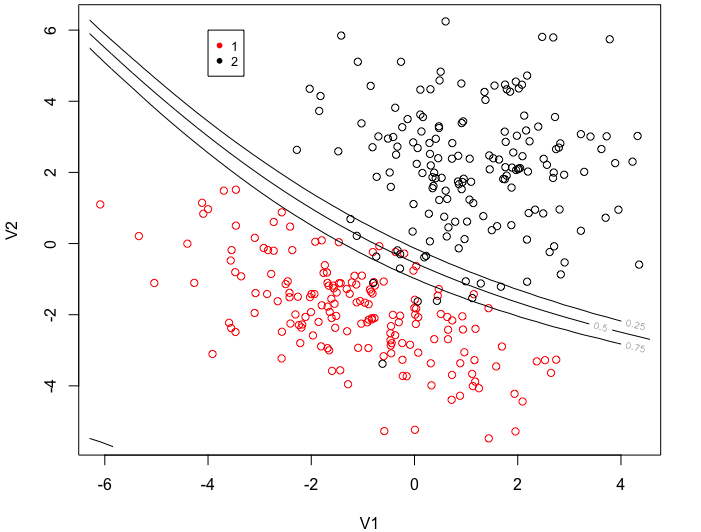
\includegraphics[width=1\linewidth]{img/front-decision-synth-1-adq}
		\caption{\small A.D. Quadratique}
		\label{fig:front-decision-synth-1-adq}%
	\end{subfigure}%
	\begin{subfigure}[b]{0.45\linewidth}
		\centering
		\captionsetup{justification=centering, margin=1cm}
		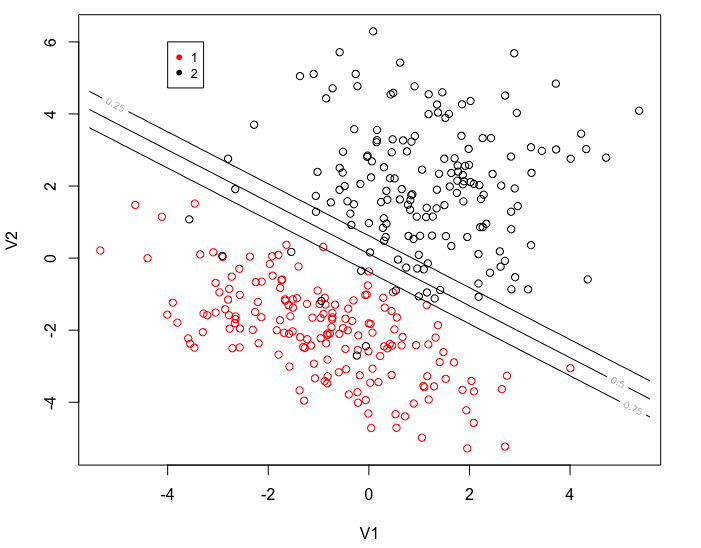
\includegraphics[width=1\linewidth]{img/front-decision-synth-1-adl}
		\caption{\small A.D. Linaire}
		\label{fig:front-decision-synth-1-adl}%
	\end{subfigure}\\%
	\begin{subfigure}[b]{0.45\linewidth}
		\centering
		\captionsetup{justification=centering, margin=1cm}
		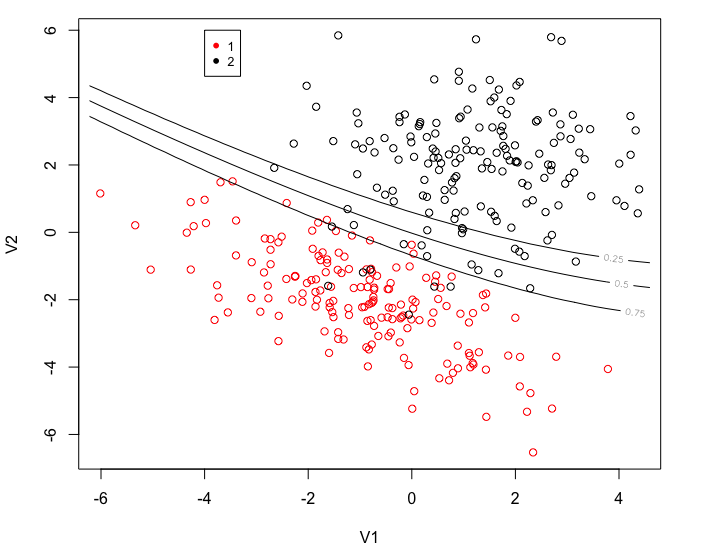
\includegraphics[width=1\linewidth]{img/front-decision-synth-1-nba}
		\caption{\small Bayésien naïf}
		\label{fig:front-decision-synth-1-nba}%
	\end{subfigure}%
	\begin{subfigure}[b]{0.45\linewidth}
		\centering
		\captionsetup{justification=centering, margin=1cm}
		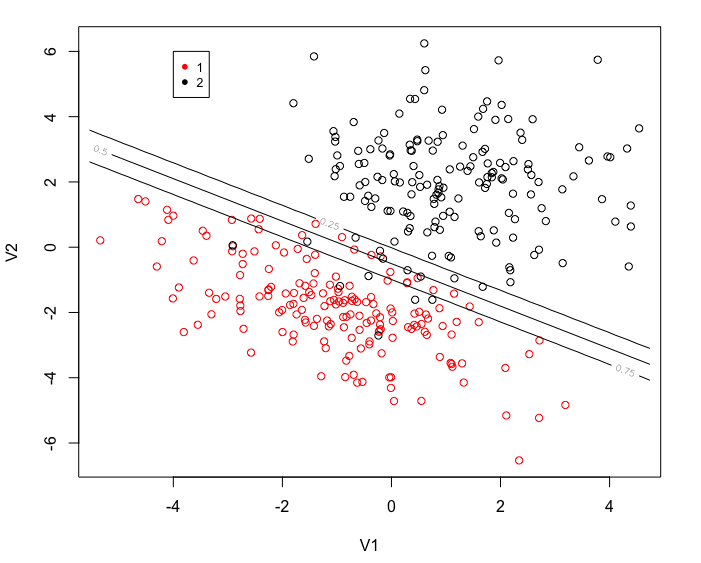
\includegraphics[width=1\linewidth]{img/front-decision-synth-1-reg-log}
		\caption{\small Régression logistique}
		\label{fig:front-decision-synth-1-reg-log}%
	\end{subfigure}\\%
	\begin{subfigure}[b]{0.45\linewidth}
		\centering
		\captionsetup{justification=centering, margin=1cm}
		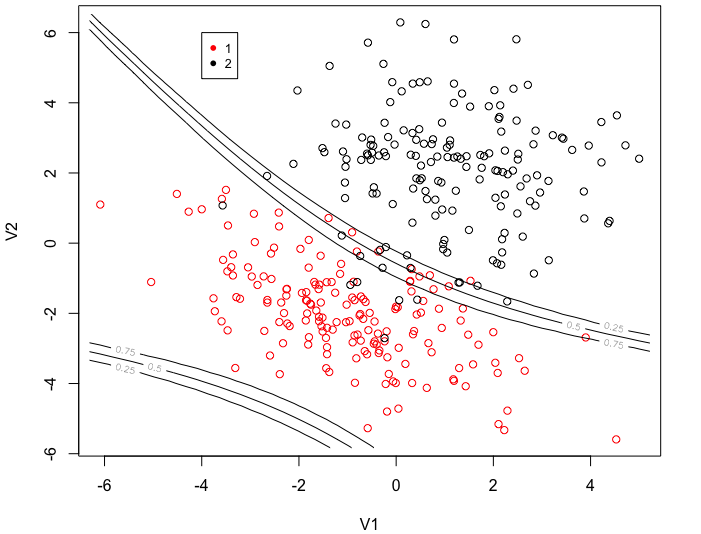
\includegraphics[width=1\linewidth]{img/front-decision-synth-1-reg-log-quad}
		\caption{\small Régression logistique quadratique}
		\label{fig:front-decision-synth-1-reg-log-quad}%
	\end{subfigure}%
	\begin{subfigure}[b]{0.45\linewidth}
		\centering
		\captionsetup{justification=centering, margin=1cm}
		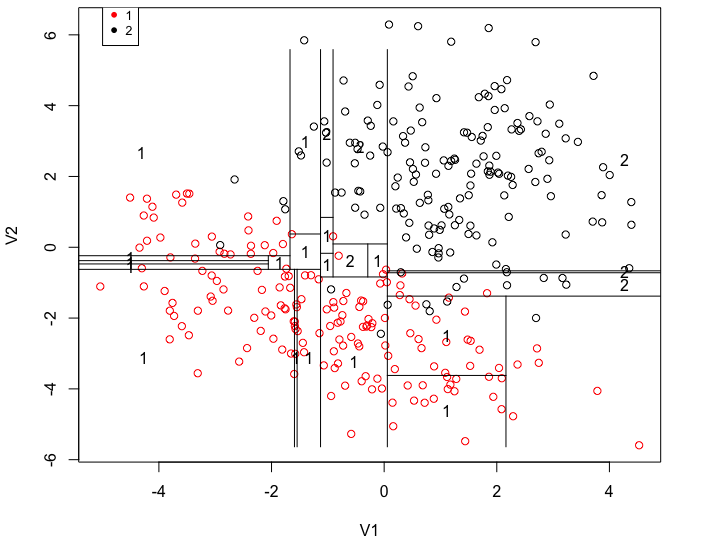
\includegraphics[width=1\linewidth]{img/front-decision-synth-1-tree}
		\caption{\small Arbre de décision}
		\label{fig:front-decision-synth-1-tree}%
	\end{subfigure}%
	\caption{\small Frontières de décision des classifieurs pour les données \textit{Synth1} au niveaux $\mathbb{P}(\omega_1|x) = \{0.25, 0.5, 0.75\}$}
	\label{fig:front-decision-synth-1}%
\end{figure}

\section{Données \textit{Synth2}}
\label{appendix:front-decision-synth-2}

\begin{figure}[H]
	\centering
	\captionsetup{justification=centering, margin=2cm}
	\begin{subfigure}[b]{0.45\linewidth}
		\centering
		\captionsetup{justification=centering, margin=1cm}
		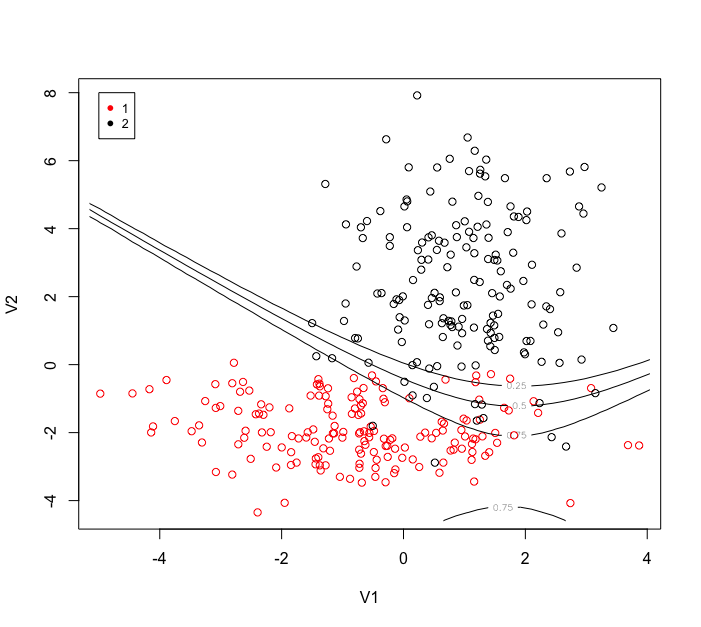
\includegraphics[width=1\linewidth]{img/front-decision-synth-2-adq}
		\caption{\small A.D. Quadratique}
		\label{fig:front-decision-synth-2-adq}%
	\end{subfigure}%
	\begin{subfigure}[b]{0.45\linewidth}
		\centering
		\captionsetup{justification=centering, margin=1cm}
		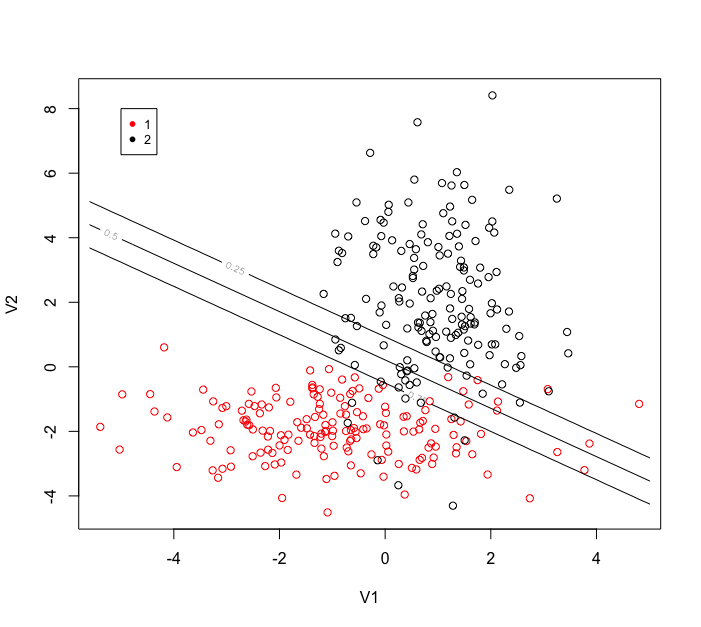
\includegraphics[width=1\linewidth]{img/front-decision-synth-2-adl}
		\caption{\small A.D. Linaire}
		\label{fig:front-decision-synth-2-adl}%
	\end{subfigure}\\%
	\begin{subfigure}[b]{0.45\linewidth}
		\centering
		\captionsetup{justification=centering, margin=1cm}
		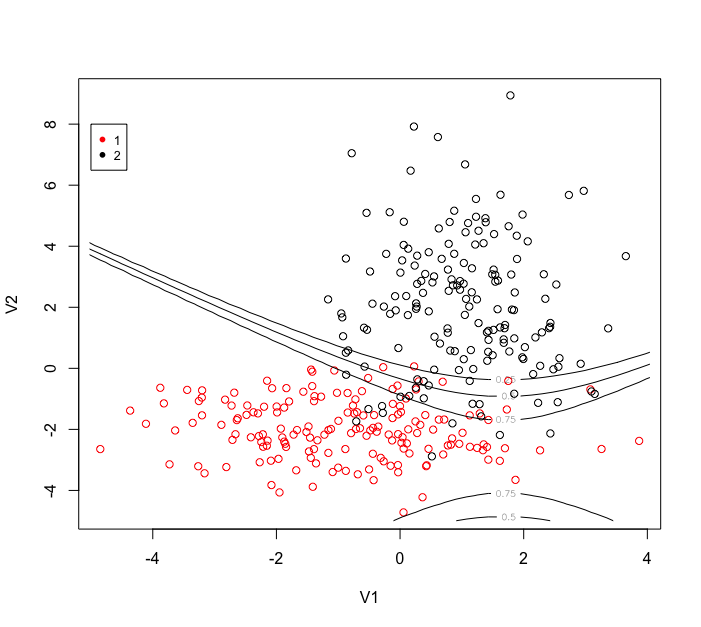
\includegraphics[width=1\linewidth]{img/front-decision-synth-2-nba}
		\caption{\small Bayésien naïf}
		\label{fig:front-decision-synth-2-nba}%
	\end{subfigure}%
	\begin{subfigure}[b]{0.45\linewidth}
		\centering
		\captionsetup{justification=centering, margin=1cm}
		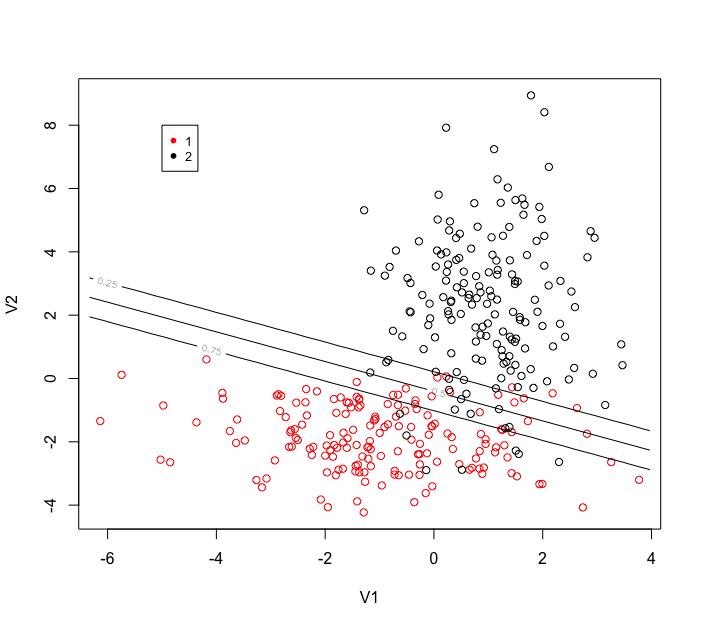
\includegraphics[width=1\linewidth]{img/front-decision-synth-2-reg-log}
		\caption{\small Régression logistique}
		\label{fig:front-decision-synth-2-reg-log}%
	\end{subfigure}\\%
	\begin{subfigure}[b]{0.45\linewidth}
		\centering
		\captionsetup{justification=centering, margin=1cm}
		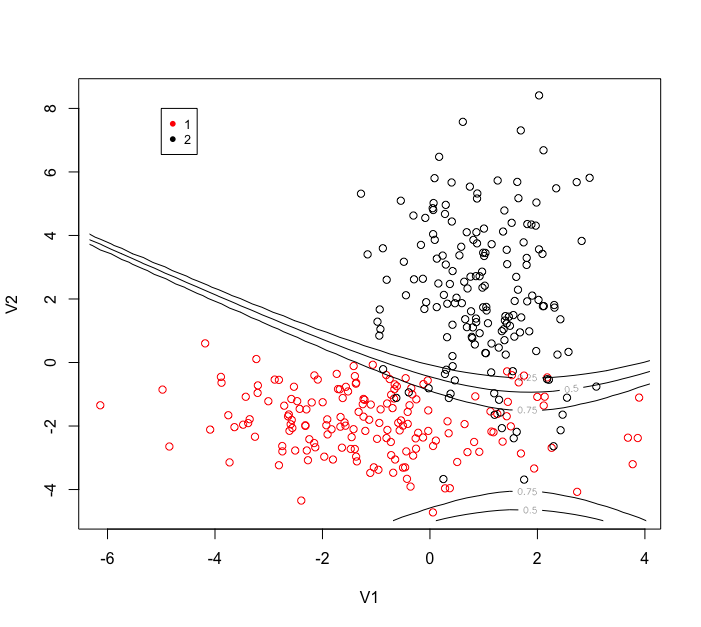
\includegraphics[width=1\linewidth]{img/front-decision-synth-2-reg-log-quad}
		\caption{\small Régression logistique quadratique}
		\label{fig:front-decision-synth-2-reg-log-quad}%
	\end{subfigure}%
	\begin{subfigure}[b]{0.45\linewidth}
		\centering
		\captionsetup{justification=centering, margin=1cm}
		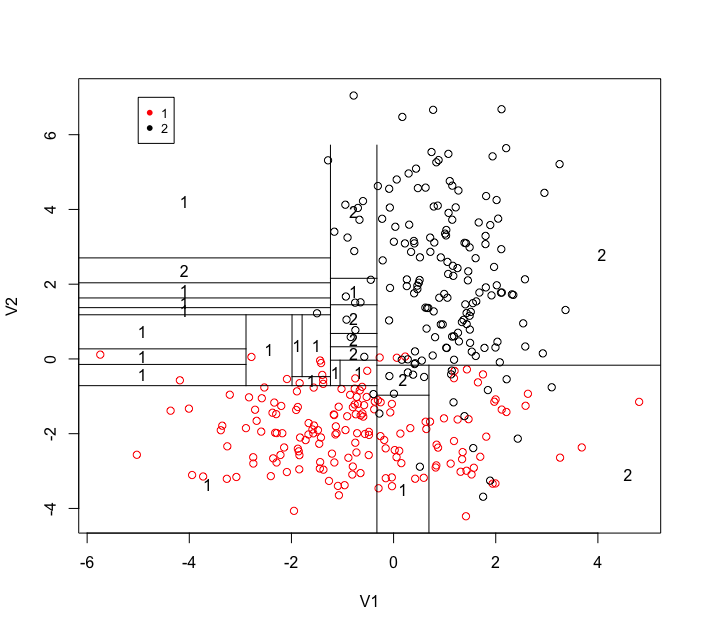
\includegraphics[width=1\linewidth]{img/front-decision-synth-2-tree}
		\caption{\small Arbre de décision}
		\label{fig:front-decision-synth-2-tree}%
	\end{subfigure}%
	\caption{\small Frontières de décision des classifieurs pour les données \textit{Synth2} au niveaux $\mathbb{P}(\omega_1|x) = \{0.25, 0.5, 0.75\}$}
	\label{fig:front-decision-synth-2}%
\end{figure}



\section{Données \textit{Synth3}}
\label{appendix:front-decision-synth-3}


\begin{figure}[H]
	\centering
	\captionsetup{justification=centering, margin=2cm}
	\begin{subfigure}[b]{0.45\linewidth}
		\centering
		\captionsetup{justification=centering, margin=1cm}
		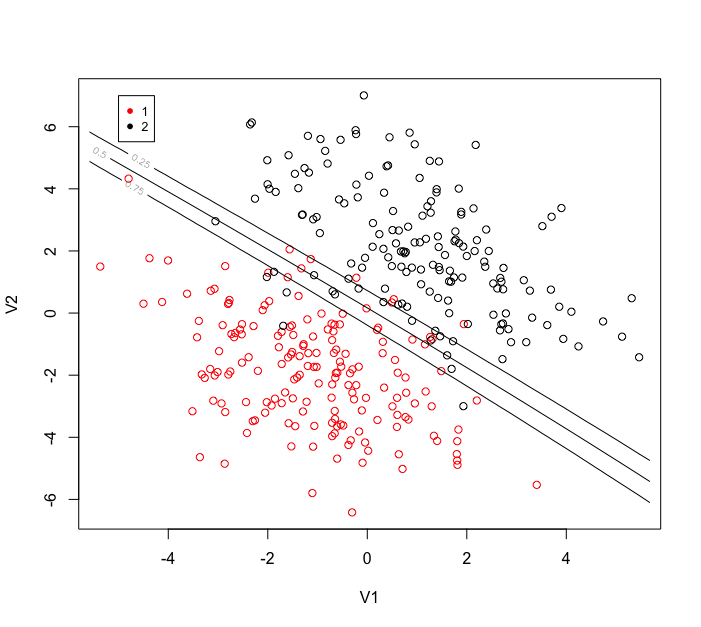
\includegraphics[width=1\linewidth]{img/front-decision-synth-3-adq}
		\caption{\small A.D. Quadratique}
		\label{fig:front-decision-synth-3-adq}%
	\end{subfigure}%
	\begin{subfigure}[b]{0.45\linewidth}
		\centering
		\captionsetup{justification=centering, margin=1cm}
		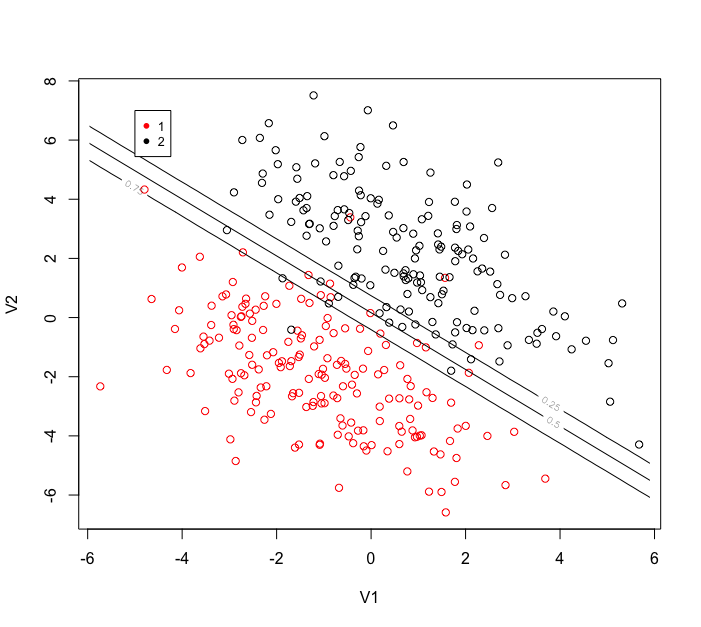
\includegraphics[width=1\linewidth]{img/front-decision-synth-3-adl}
		\caption{\small A.D. Linaire}
		\label{fig:front-decision-synth-3-adl}%
	\end{subfigure}\\%
	\begin{subfigure}[b]{0.45\linewidth}
		\centering
		\captionsetup{justification=centering, margin=1cm}
		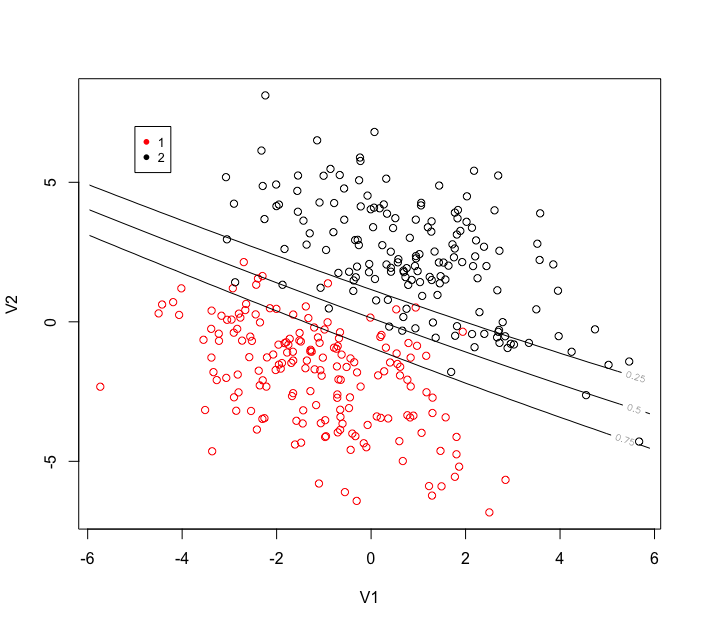
\includegraphics[width=1\linewidth]{img/front-decision-synth-3-nba}
		\caption{\small Bayésien naïf}
		\label{fig:front-decision-synth-3-nba}%
	\end{subfigure}%
	\begin{subfigure}[b]{0.45\linewidth}
		\centering
		\captionsetup{justification=centering, margin=1cm}
		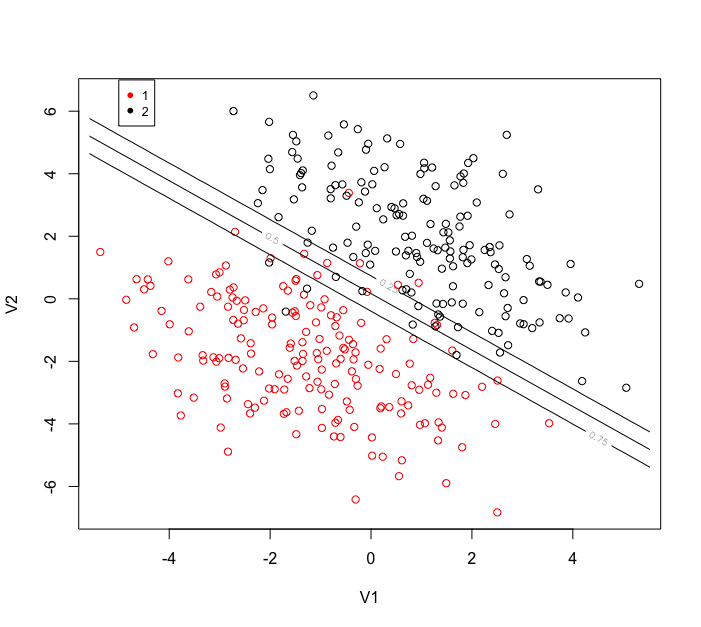
\includegraphics[width=1\linewidth]{img/front-decision-synth-3-reg-log}
		\caption{\small Régression logistique}
		\label{fig:front-decision-synth-3-reg-log}%
	\end{subfigure}\\%
	\begin{subfigure}[b]{0.45\linewidth}
		\centering
		\captionsetup{justification=centering, margin=1cm}
		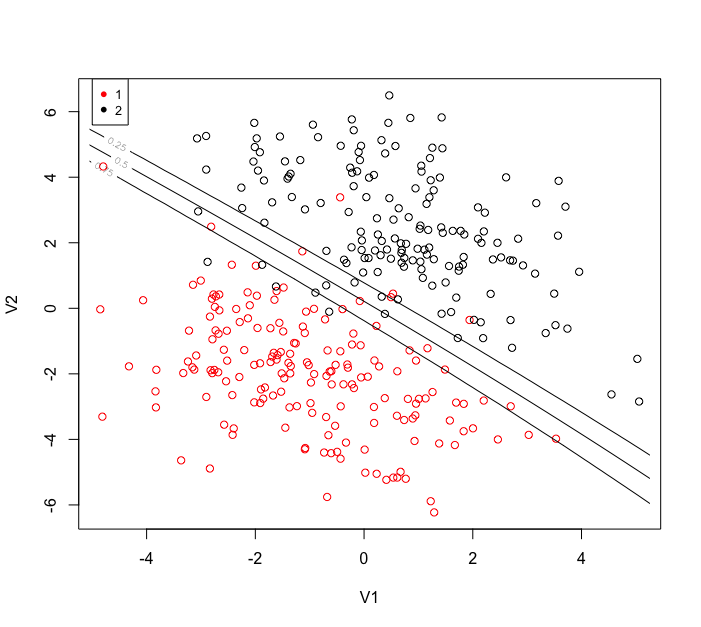
\includegraphics[width=1\linewidth]{img/front-decision-synth-3-reg-log-quad}
		\caption{\small Régression logistique quadratique}
		\label{fig:front-decision-synth-3-reg-log-quad}%
	\end{subfigure}%
	\begin{subfigure}[b]{0.45\linewidth}
		\centering
		\captionsetup{justification=centering, margin=1cm}
		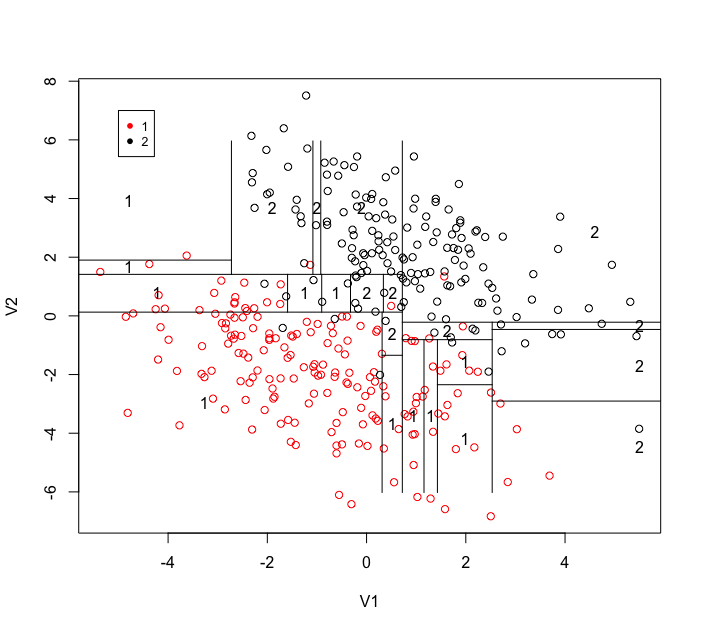
\includegraphics[width=1\linewidth]{img/front-decision-synth-3-tree}
		\caption{\small Arbre de décision}
		\label{fig:front-decision-synth-3-tree}%
	\end{subfigure}%
	\caption{\small Frontières de décision des classifieurs pour les données \textit{Synth3} au niveaux $\mathbb{P}(\omega_1|x) = \{0.25, 0.5, 0.75\}$}
	\label{fig:front-decision-synth-3}%
\end{figure}


\end{document}